\chapter{Implementation and Build}

\section{Designing and Prototyping}
We designed the prototype of the circuit on breadboards which included the microcontroller, radio module and an oled display.

We used an atmega328p microcontroller as the library we needed for the creating mesh network with NRF24L01+ radio module was available for only for it.

We added an oled display for testing and debugging purposes and is not intended to be a part of our final product.

The breadboard circuit also had a 3.3v regulator to supply the NRF radio module. 
\begin{center}
	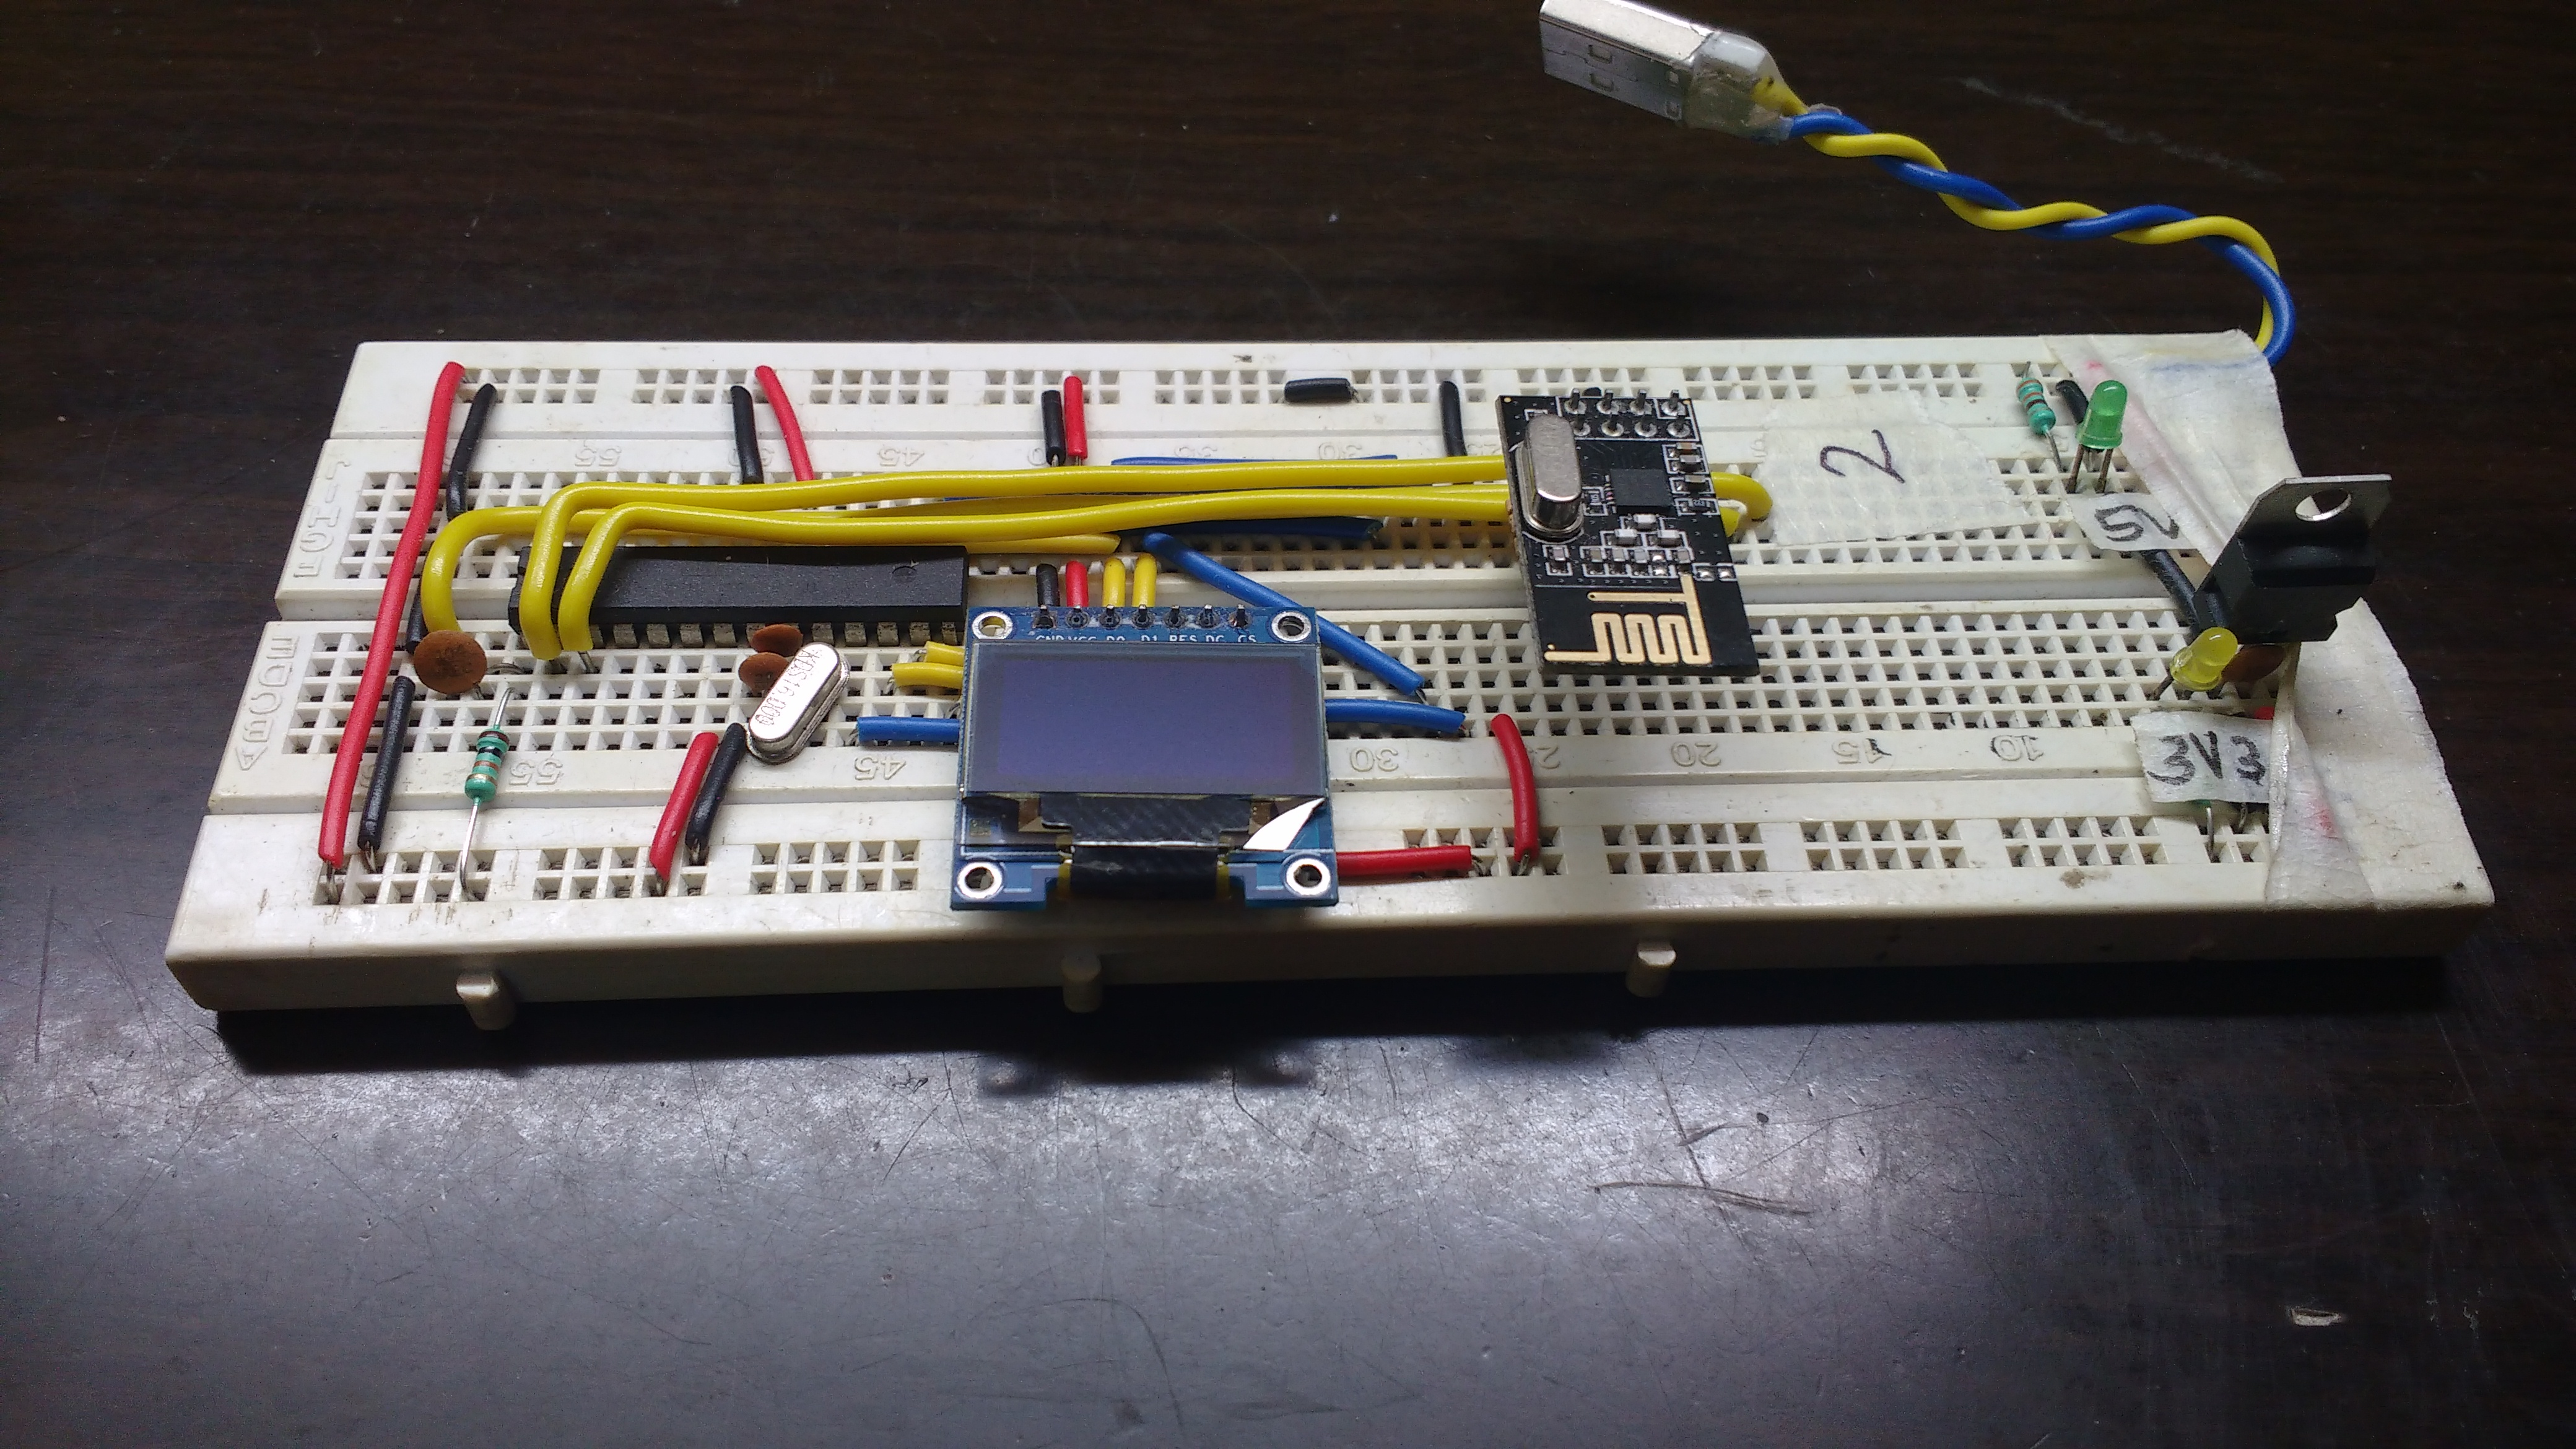
\includegraphics[scale=0.05]{Breadboard.jpg}
	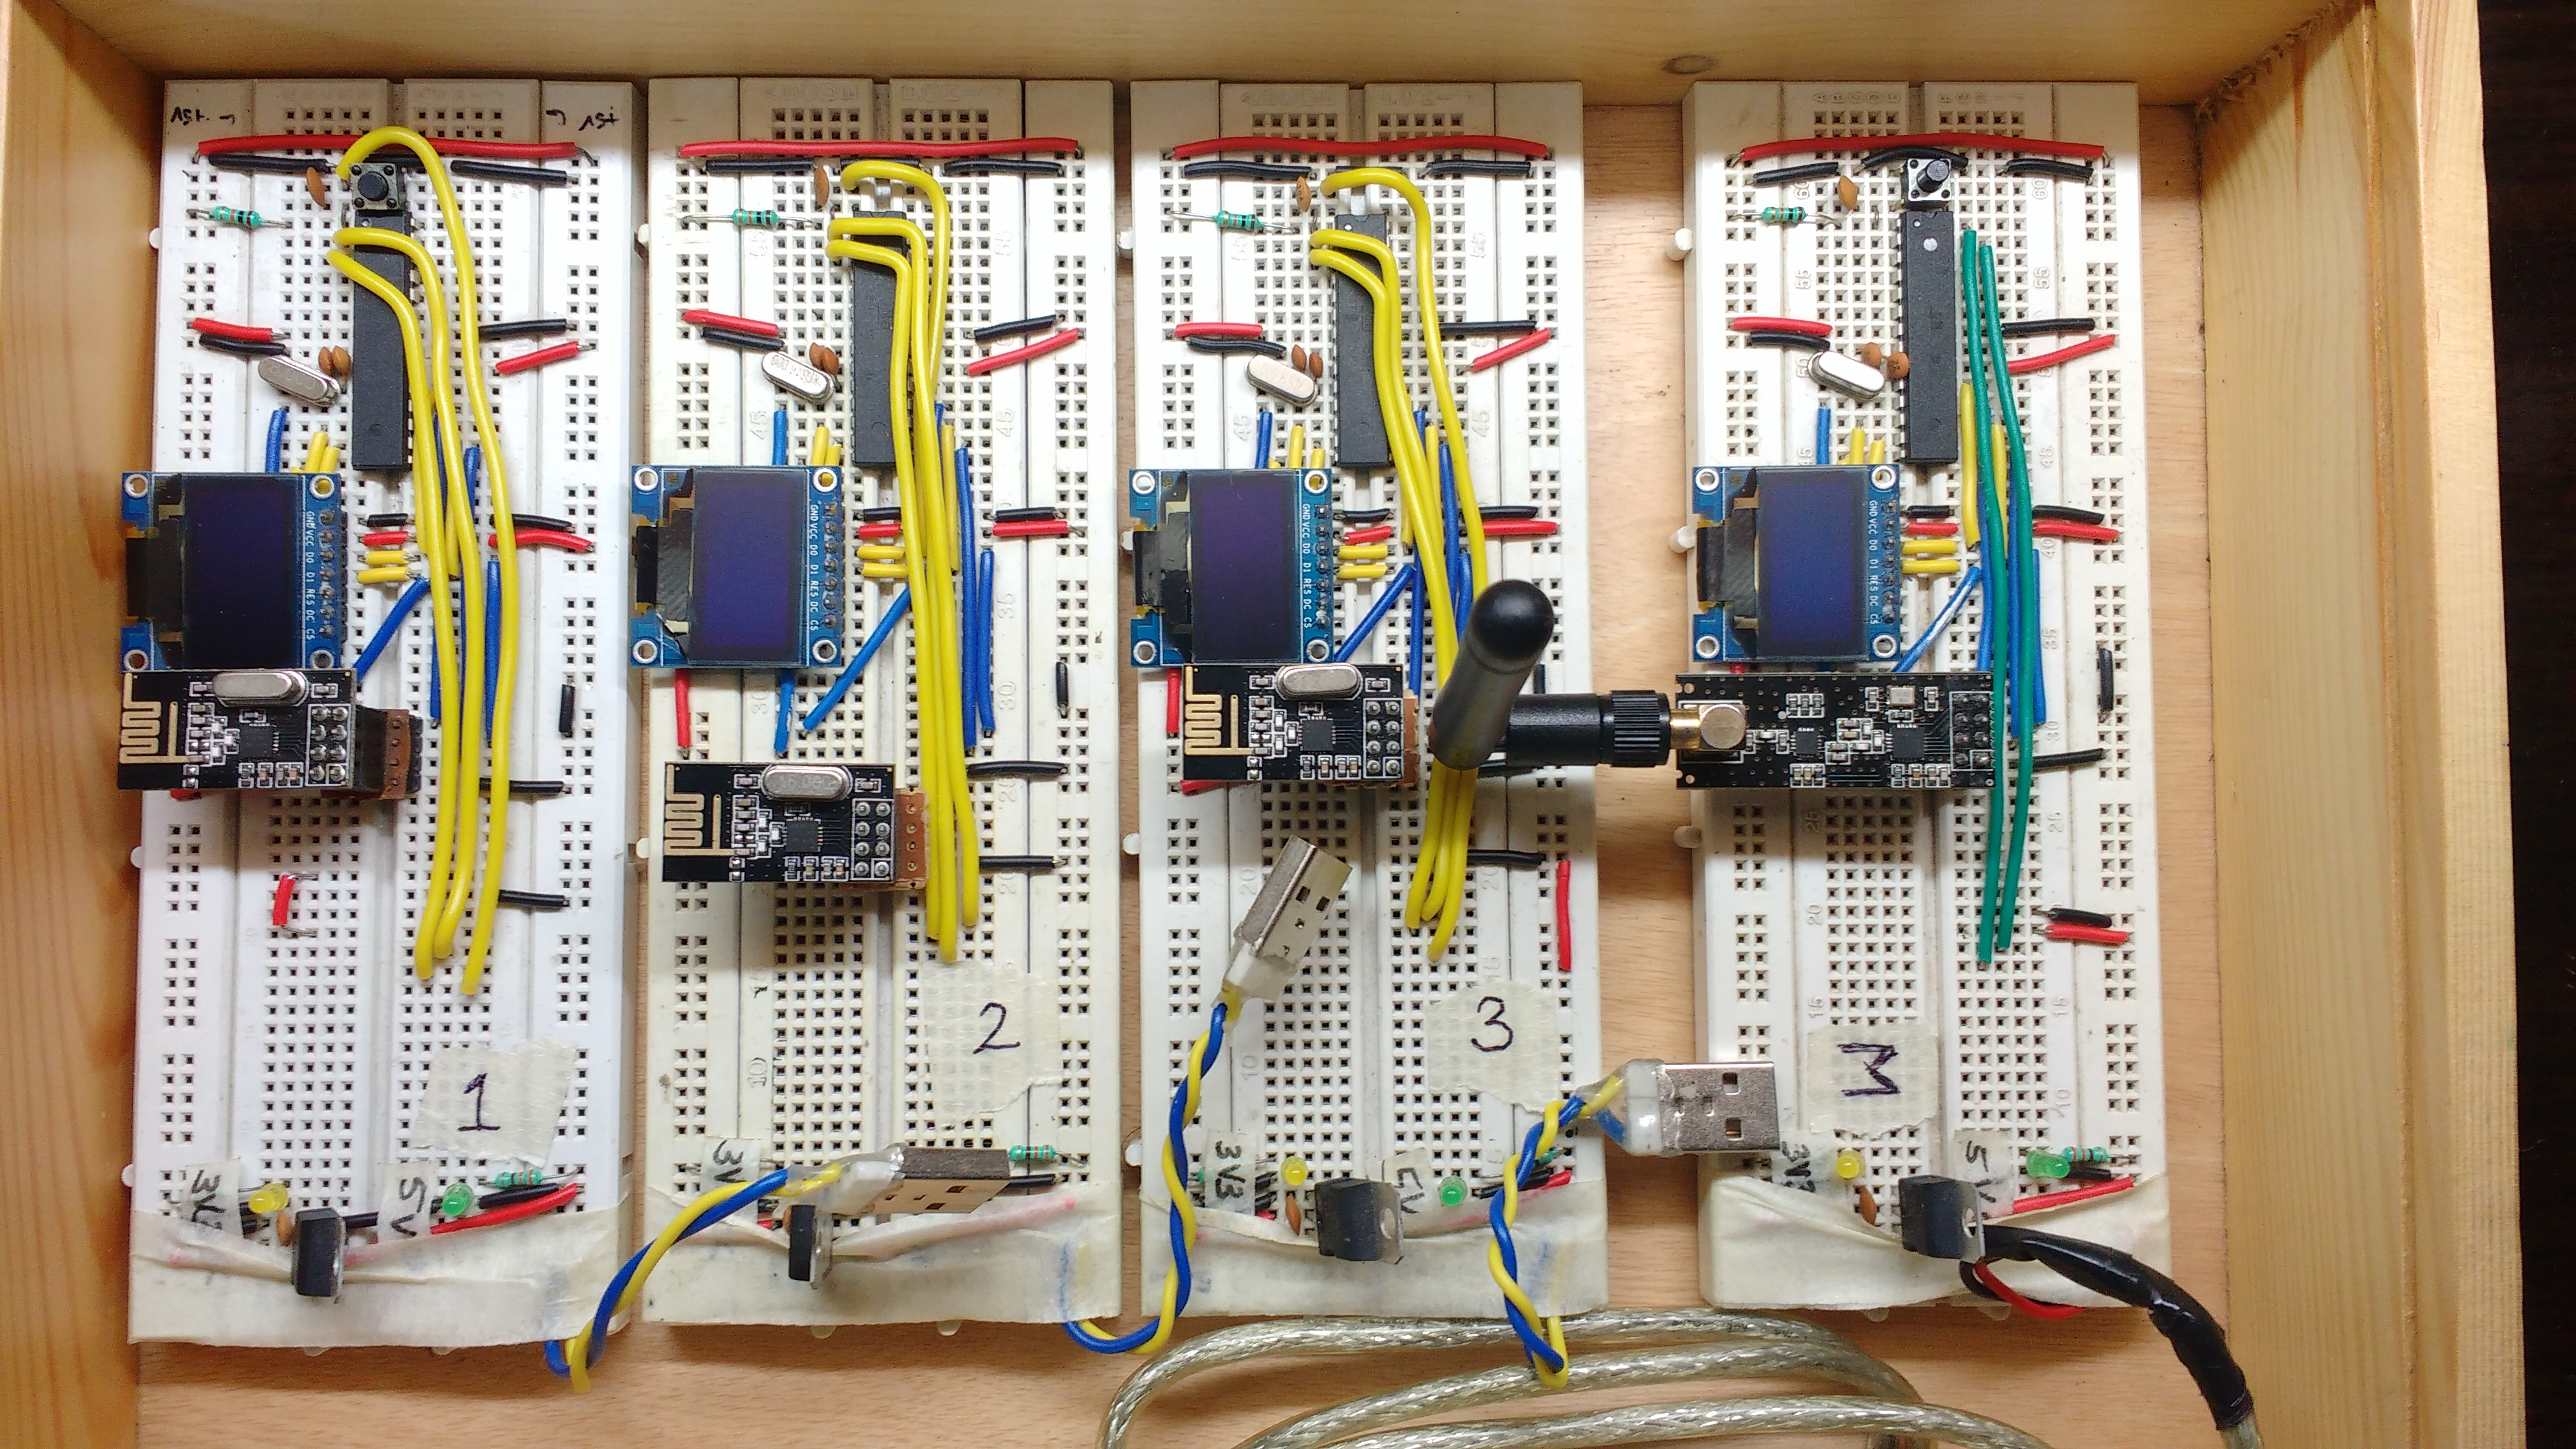
\includegraphics[scale=0.05]{Breadboard2.jpg}
\end{center}


\subsection{Radio Module Selection}
ZigBee, Lora and the NRF24L01 were the suitable choice of wireless communication modules/protocols for our project.
ZigBee offered a easy to use mesh network setup, low power consumption and robust communication protocol. But ZigBee was cost prohibitive for creating many inexpensive devices. 
Lora offered long range but had a nascent ecosystem and it too was cost prohibitive for creating many inexpensive devices. 
NRF24L01+ modules offered a decent range had a resonable networking ecosystem developed for it and was very cost effective for creating low cost modules.


\subsection{Low Power Considerations}
As we were making a battery powered device the current consumed should be as low as possible to maximize the battery life.
We required a battery life of 3-12 months before the battery needs to be replaced. Hence to reduce the active and standby current of our circuit we took the following steps.

\begin{itemize}
\item We decided to run the ATmegs328p with a clock of 8Mhz instead of the standard 16Mhz so that we can reduce the supply voltage and the current comsumption of the microcontroller. This will also reduce the number of batteries to be used as the supply voltage reduces.
\item We needed a voltage regulator to reduce and regulate the supply voltage from the battery. Standard voltage regulators like the LM117 consume 5mA operating current. Moreover the dropout voltage is too high which reduces the efficiency and also increases the voltage needed to be supplied to the device hence increasing the number of batteries.
We decided to use TC1014-3.0V which is a low dropout voltage, low quiecent current voltage regulator. This enabled our standby current to the device to be as low as 17uA and it reduced the dropout voltage to 200mV.
We purchaced the voltage regulators online from \url{tanotis.com}.
\item When the device is not transmitting the microcontroller and the radio module go into a deep sleep state. The current consumption reduces to 150uA. 50uA is used by the PIR sensor when motion is not detected. 
When motion is detected the device wakes up from its deep sleep state using interrupts and then transmits the required information and goes back to its deep sleep state. During this state the current consumption increases to 18mA for a fraction of a second before the device goes bak to sleep. out of these 18mA, 12mA is used by the NRF module and the rest by the ATmega microcontroller.
\end{itemize}

\section{PCB Design}
The board has the following features
\begin{itemize}
	\item Programming interface for both serial (Arduino) as well as ISP programming
	\item Headers for RTC, NRF radio module and Oled display
	\item Onboard LDO and ultra low quiescent current voltage regulator for battery supply (TC1014-3.0V)
\end{itemize}

We used the smallest footprint components which was practical to hand assemble so that we could make the device smaller. All the resistors and capacitors are of 0805 package, ATmega is TQFP package, the voltage regulator is SOT-5 package.
We needed to make multiple such boards.
Hence for these reasons we decided to get the PCBs professionally manufactured from a PCB prototyping service (PCBway.com).

\begin{center}
	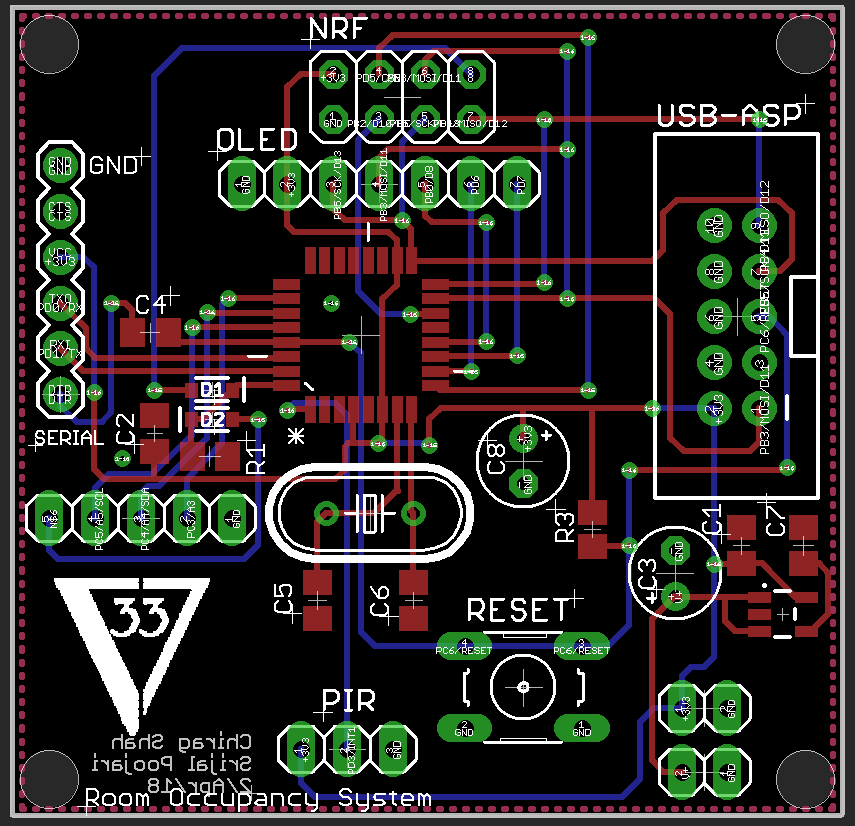
\includegraphics[scale=0.31]{EaglePCB.png}
	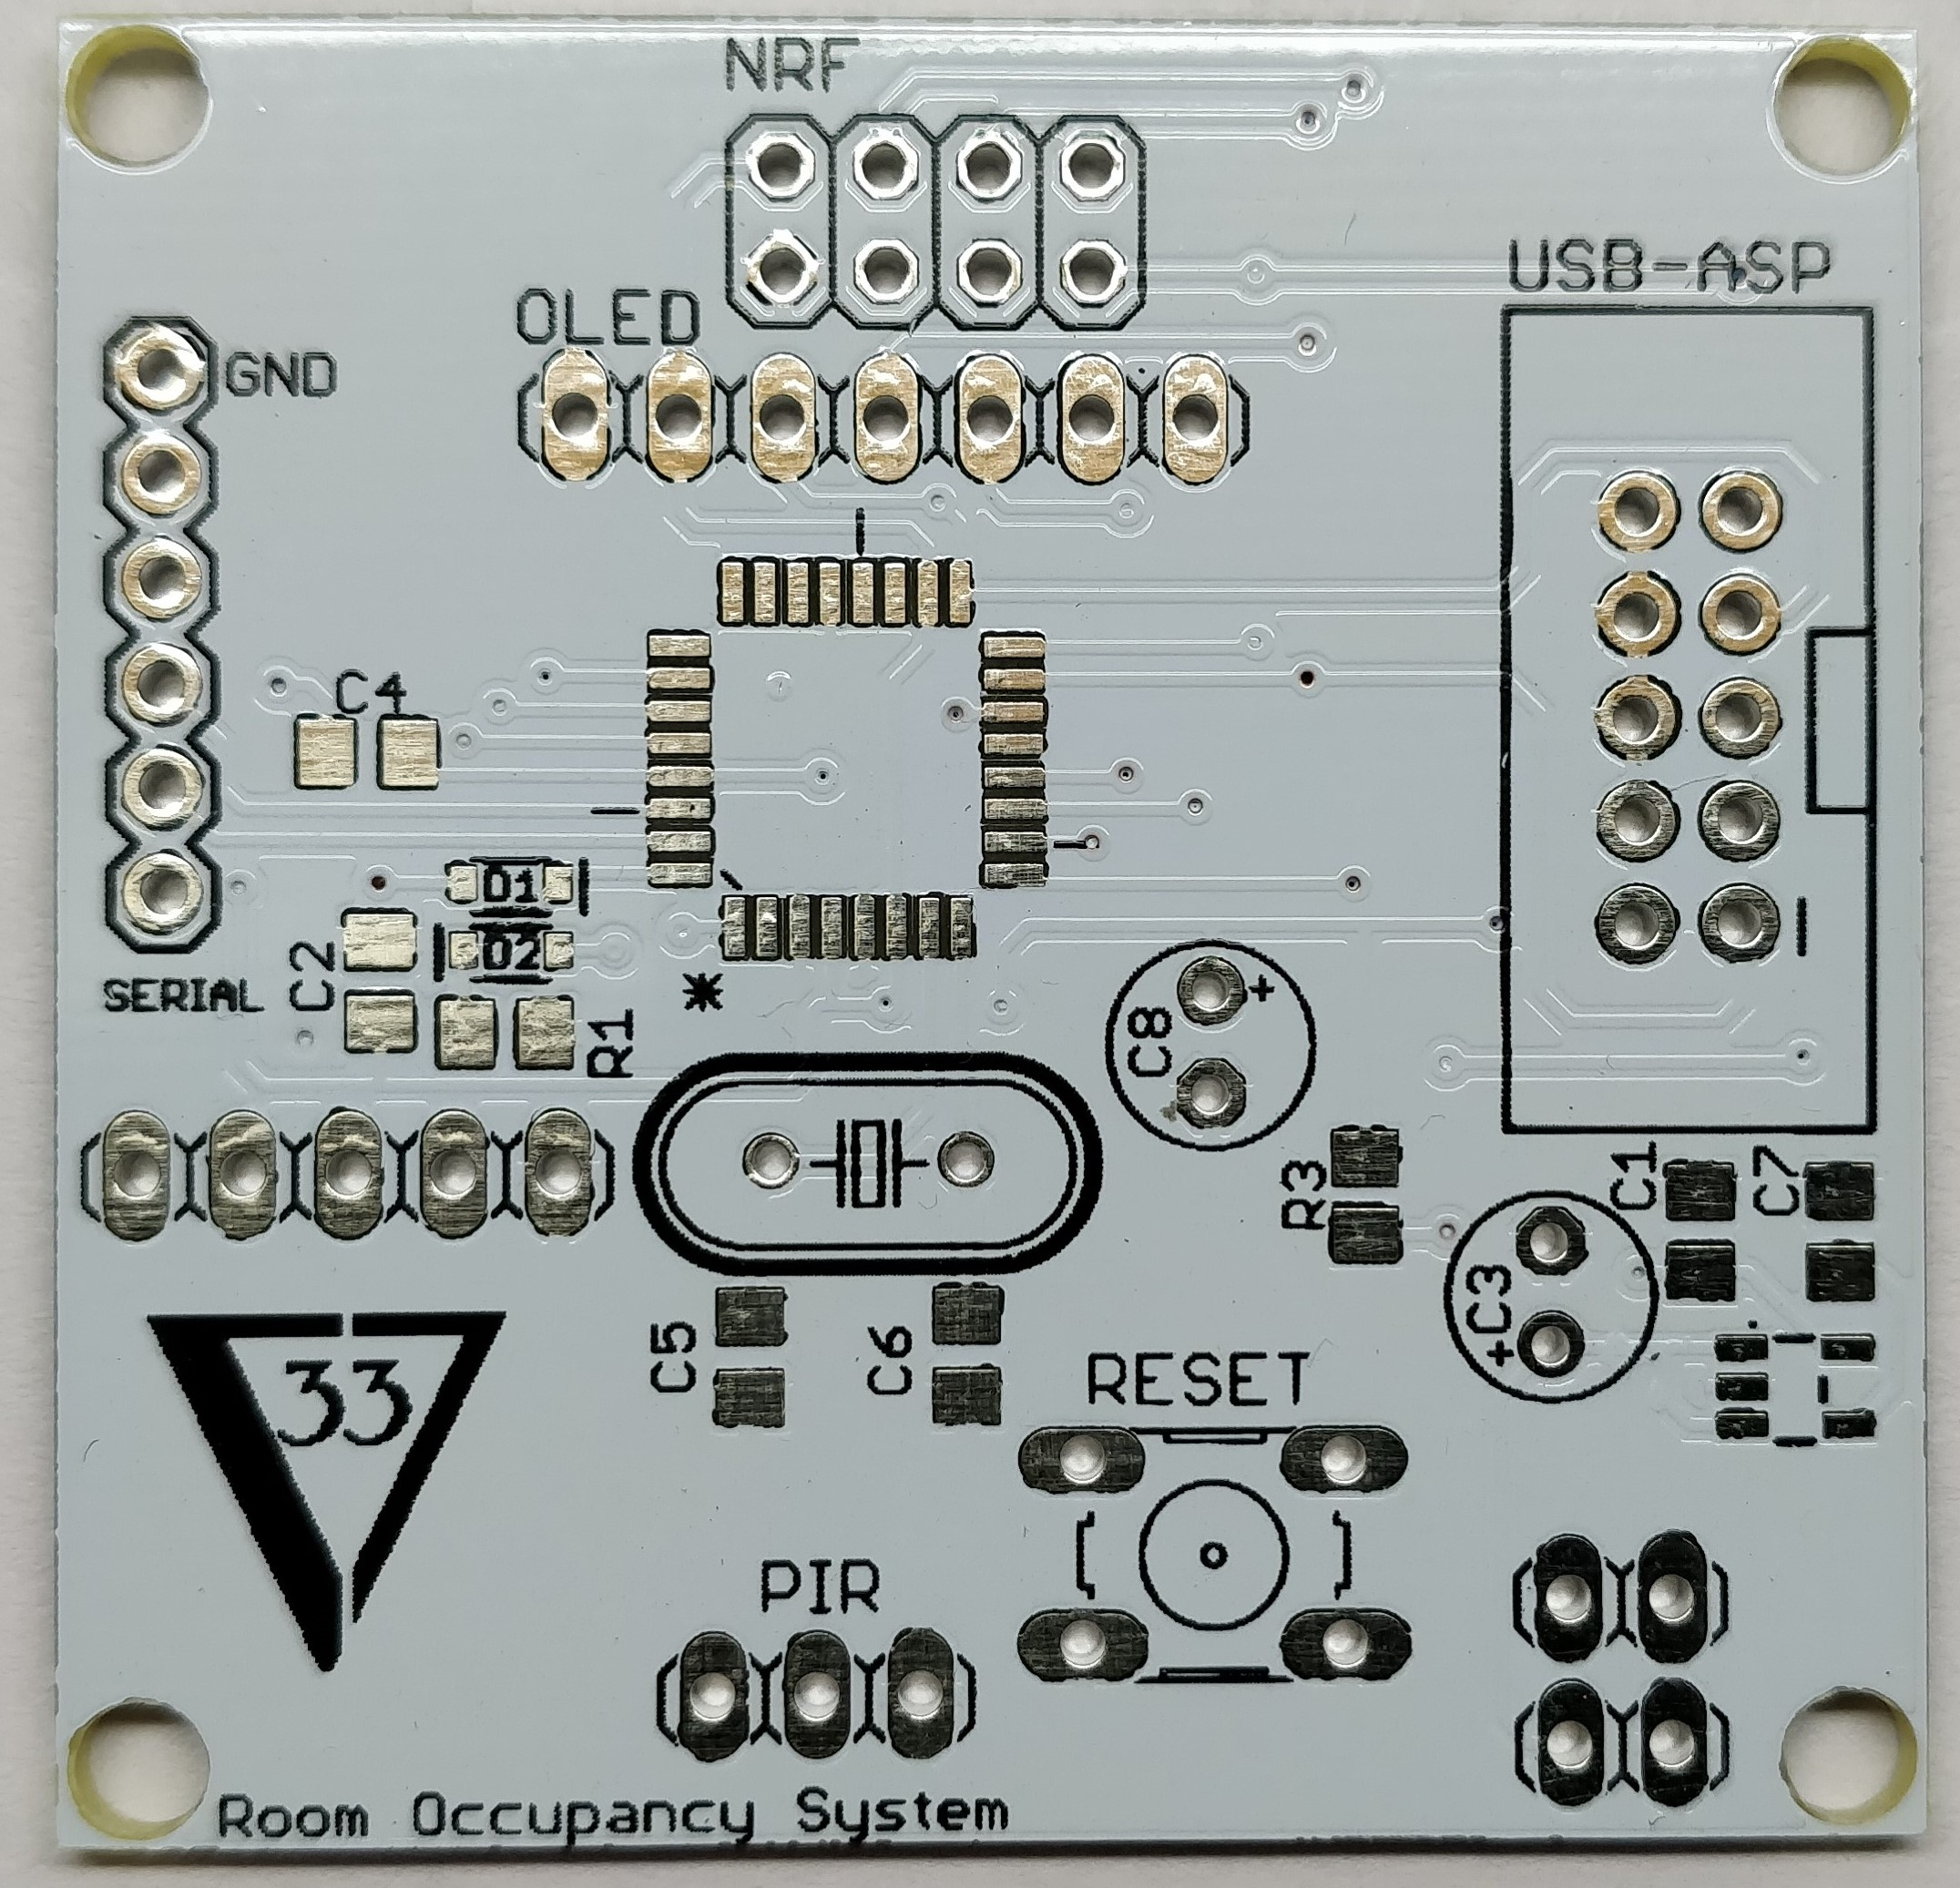
\includegraphics[scale=0.075]{PCB_1.jpg}
	
	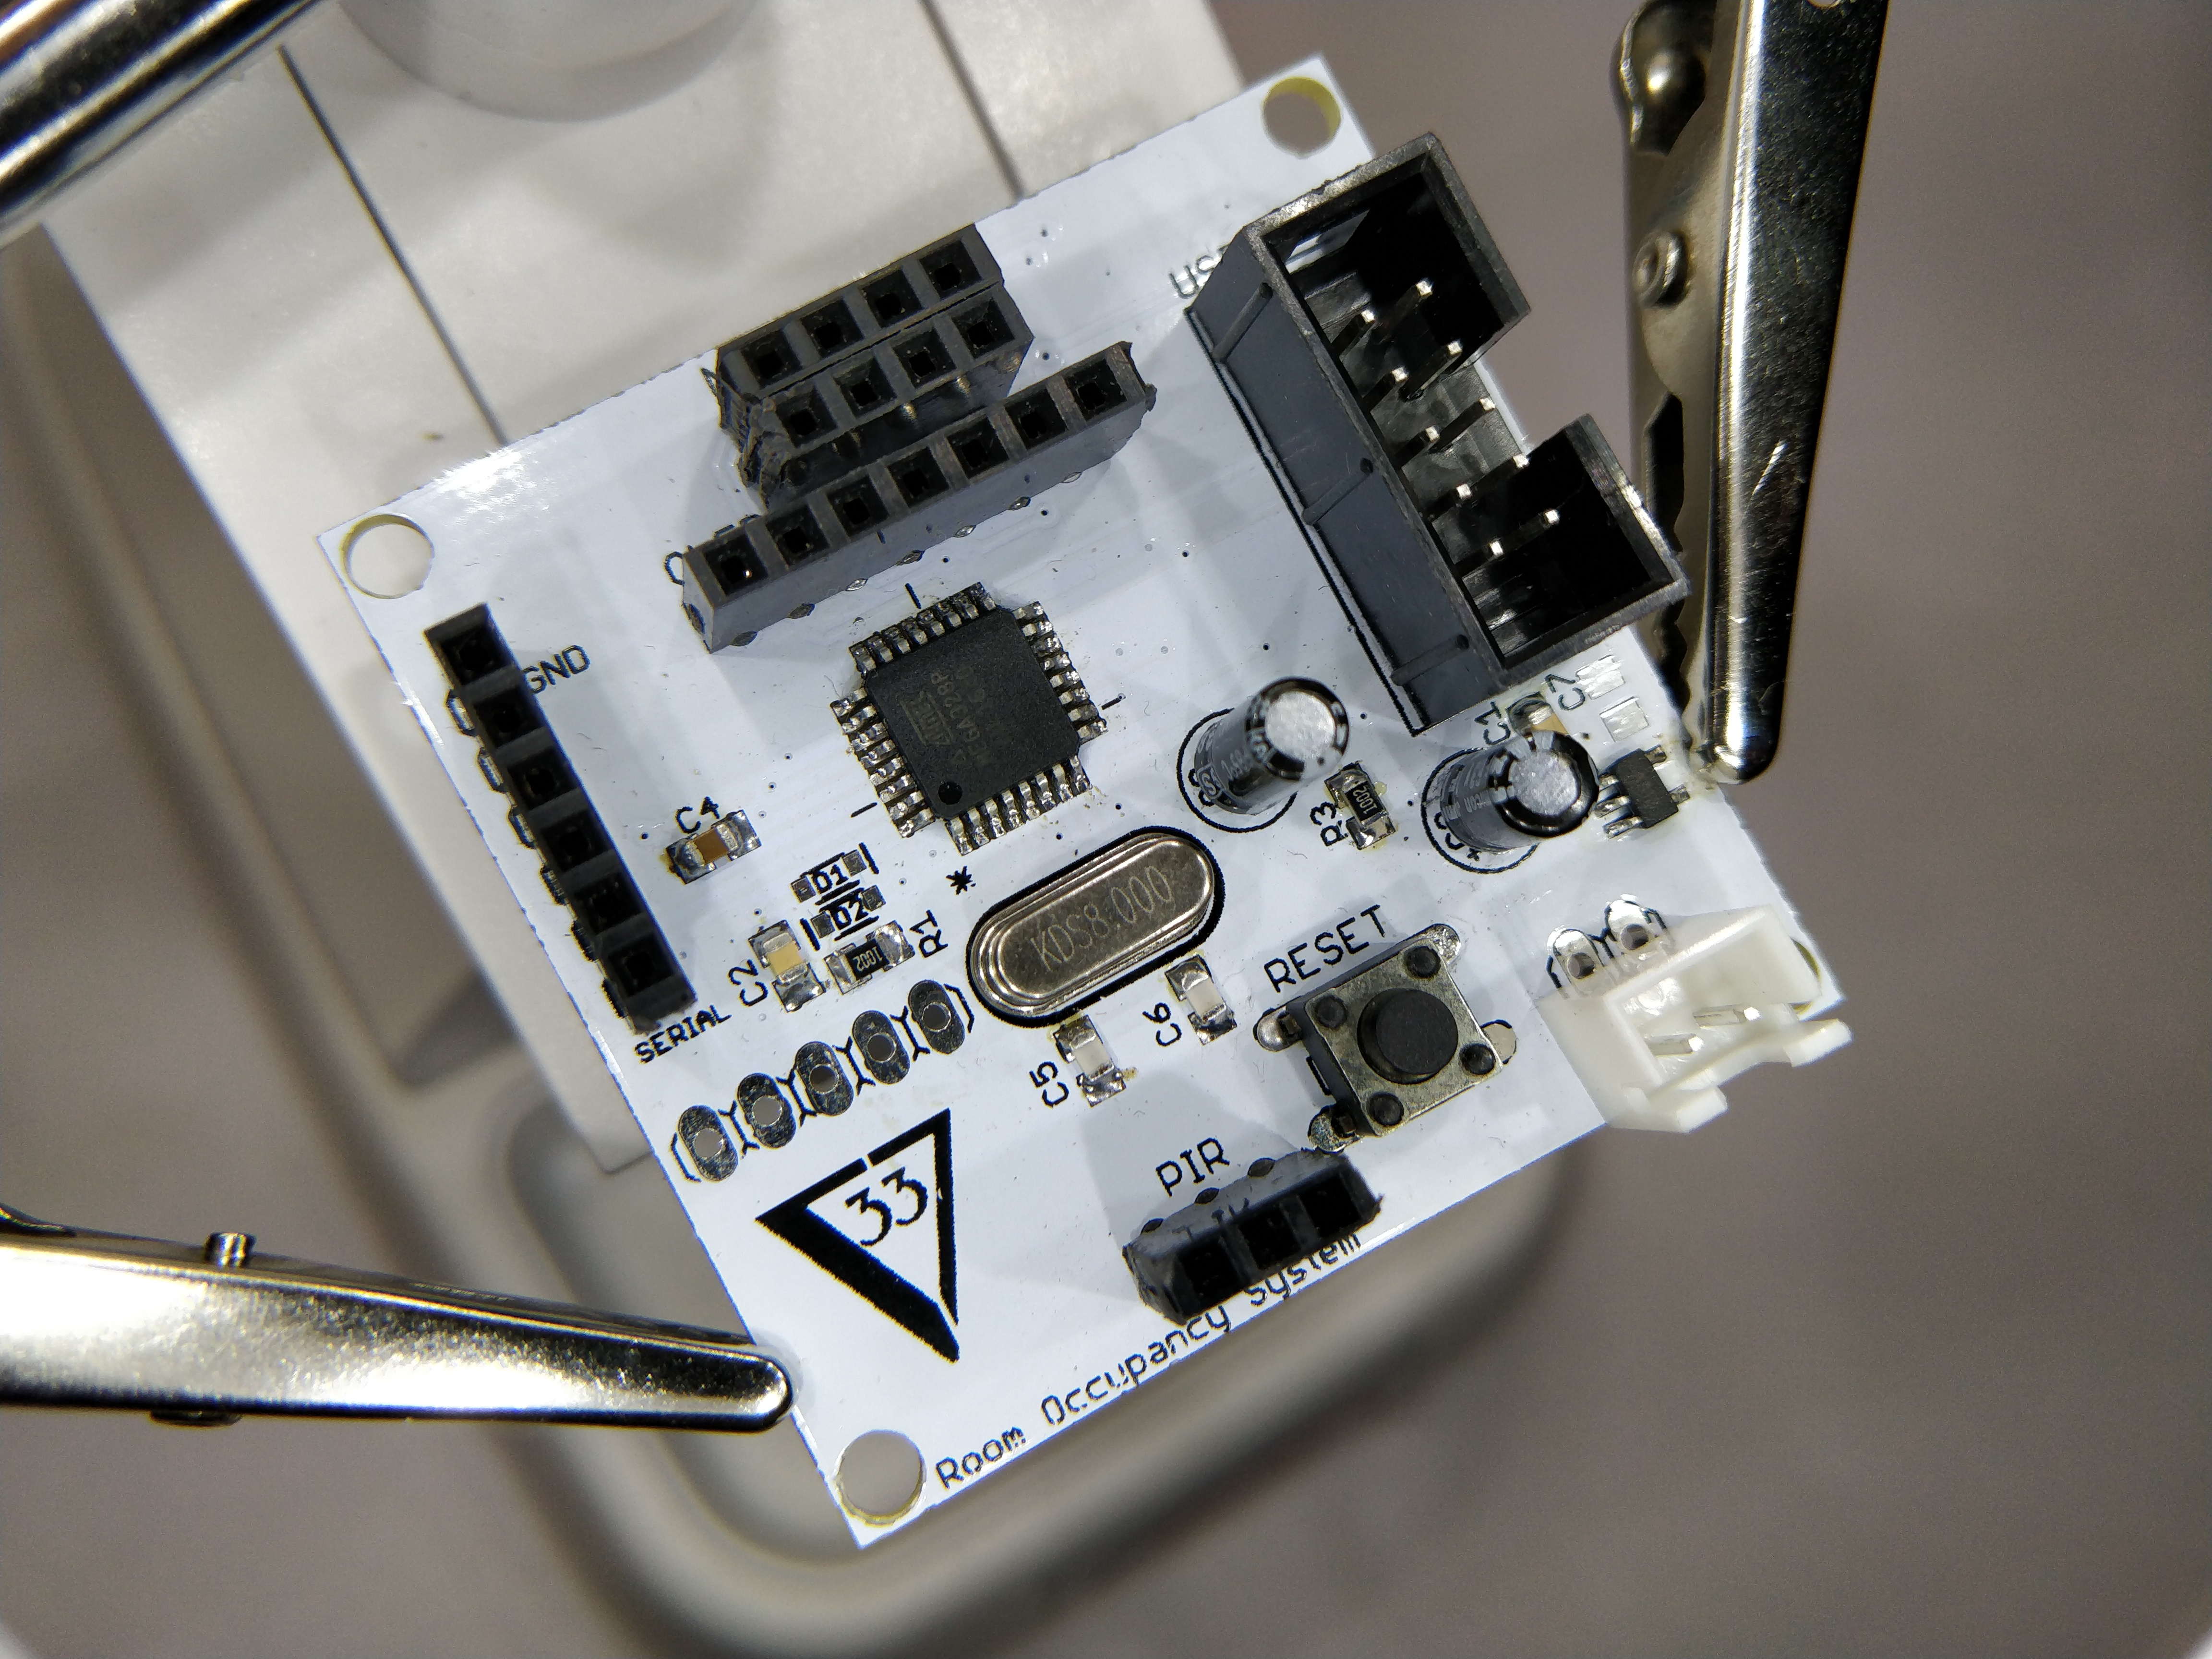
\includegraphics[scale=0.05]{PCB_2.jpg}
	\includegraphics[scale=0.05]{PCB_3.jpg}
	\\
	\vspace{10pt}
	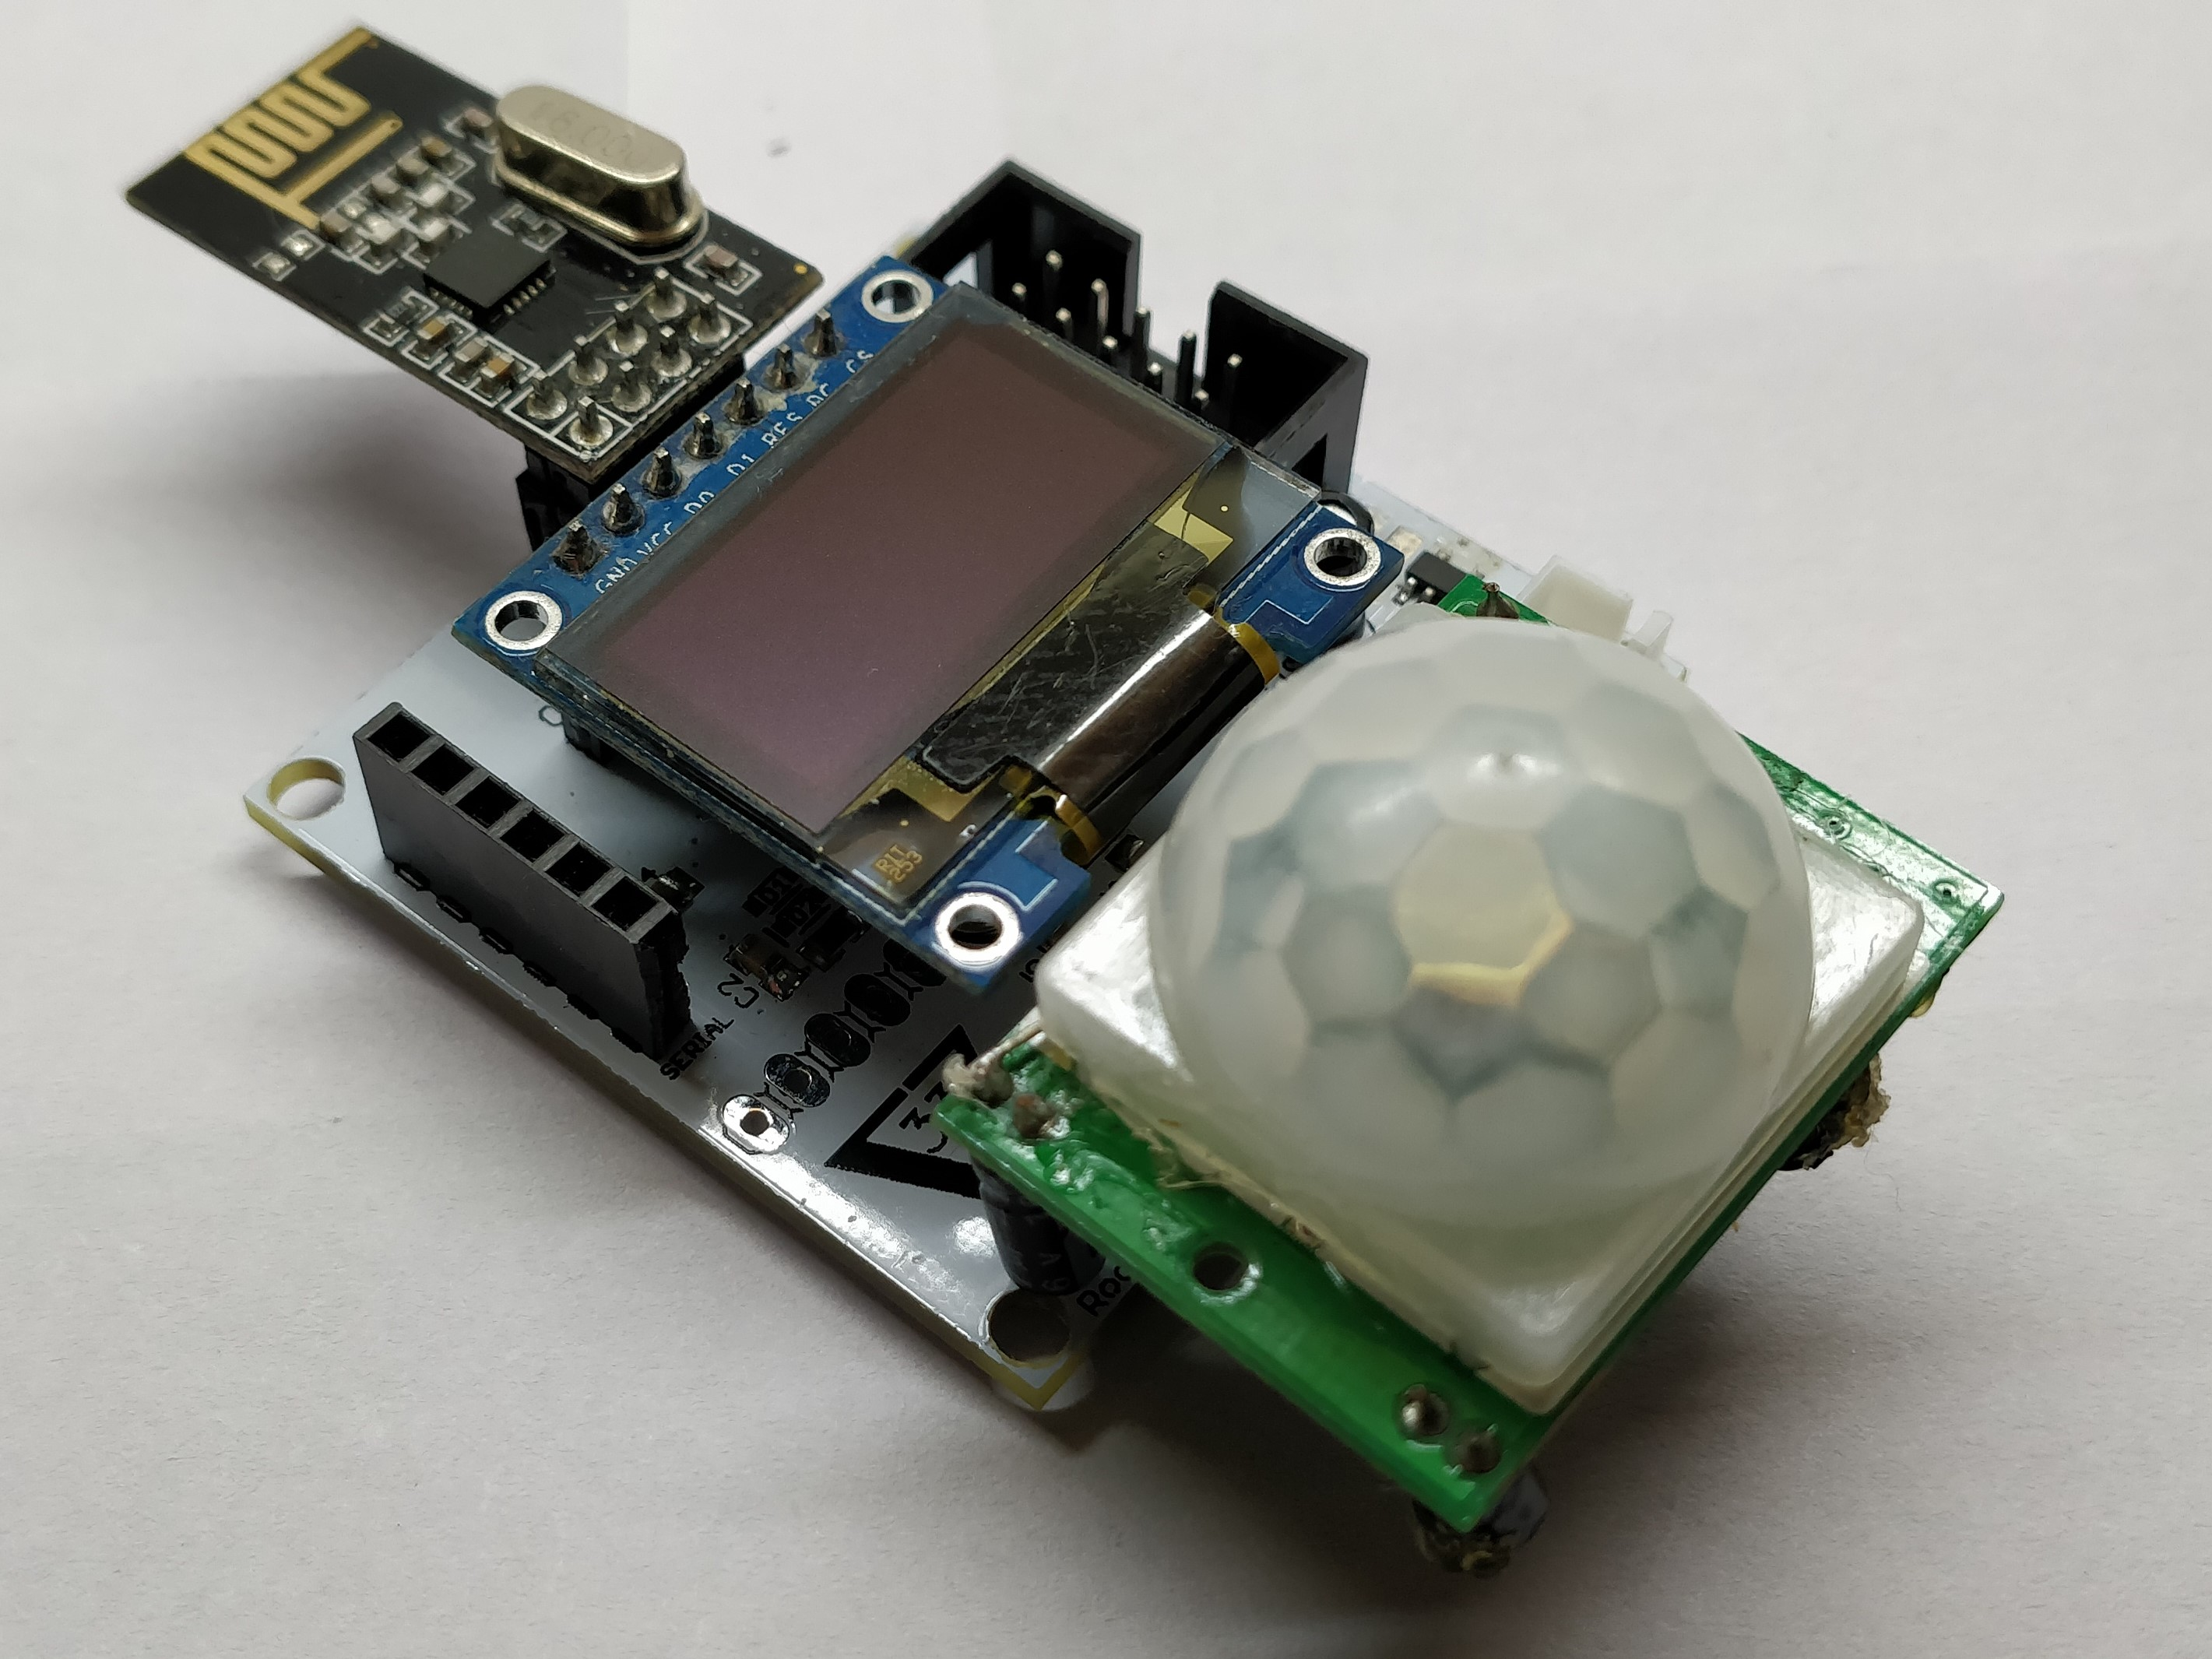
\includegraphics[scale=0.09]{AssemPCB1.jpg}
\end{center}


\section{3D Modelling and Print}
Any electronics project is incomplete without a proper enclosure to go with it. Normally we would have built something manually out of acrylic sheets or cardboard, but recently the institute had purchased a 3D printer, and we had multiple nodes to work with, so 3D printing an enclosure was the best option. 
We designed the 3D models by mainly taking the PCB, RF module and battery into consideration and tried to fit it a small form-factor. The modelling was done on Autodesk Fusion 360 from ground up. Pre-made models of the battery and PIR sensor was found on grabcad.com, which made the modelling process a bit easier.
After the design process, the model was exported as .stl files and sent to the printer for 3D printing. The first print of the base part failed due to a nozzle clog in the 3D printer. The second print was a success and the print turned out well, with all components falling in perfectly. Next we went ahead and printed the top half of the enclosure and it was a success as well.

\begin{center}
	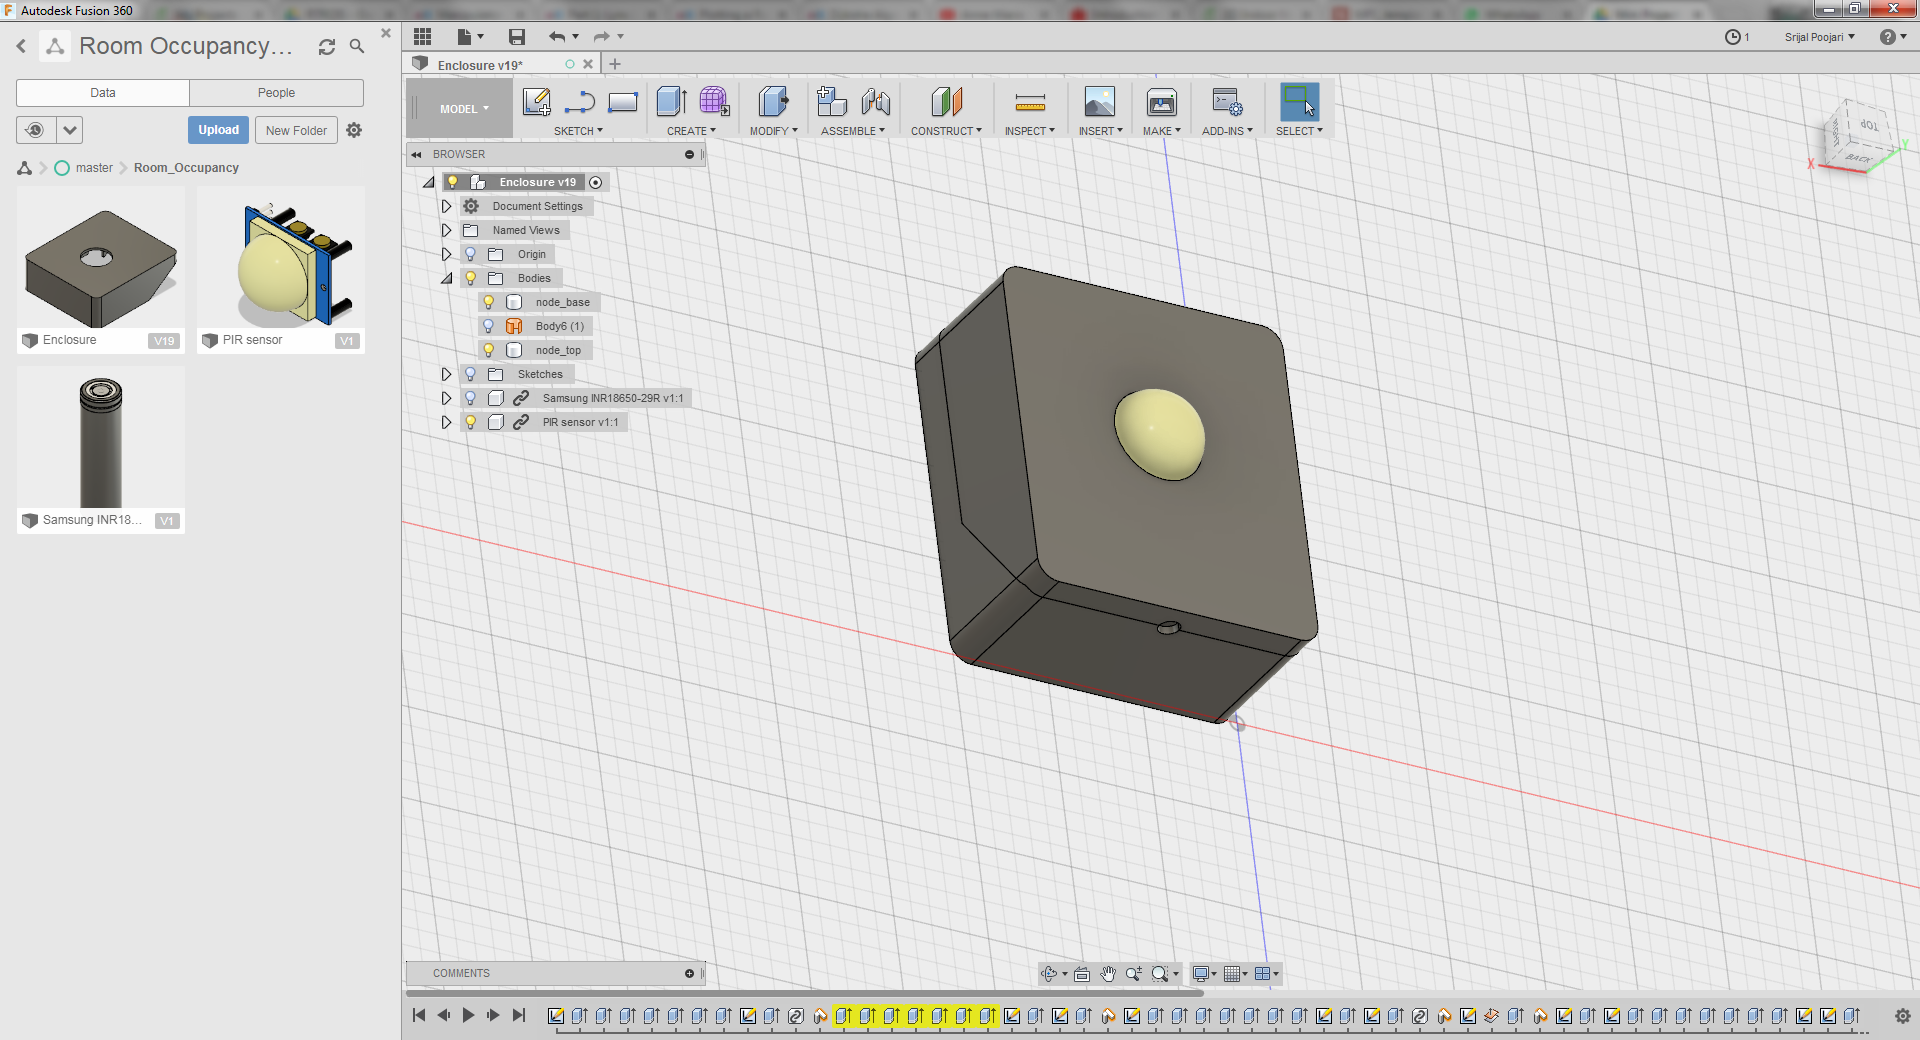
\includegraphics[scale=0.25]{model.png}
	\\
	\vspace{10pt}
	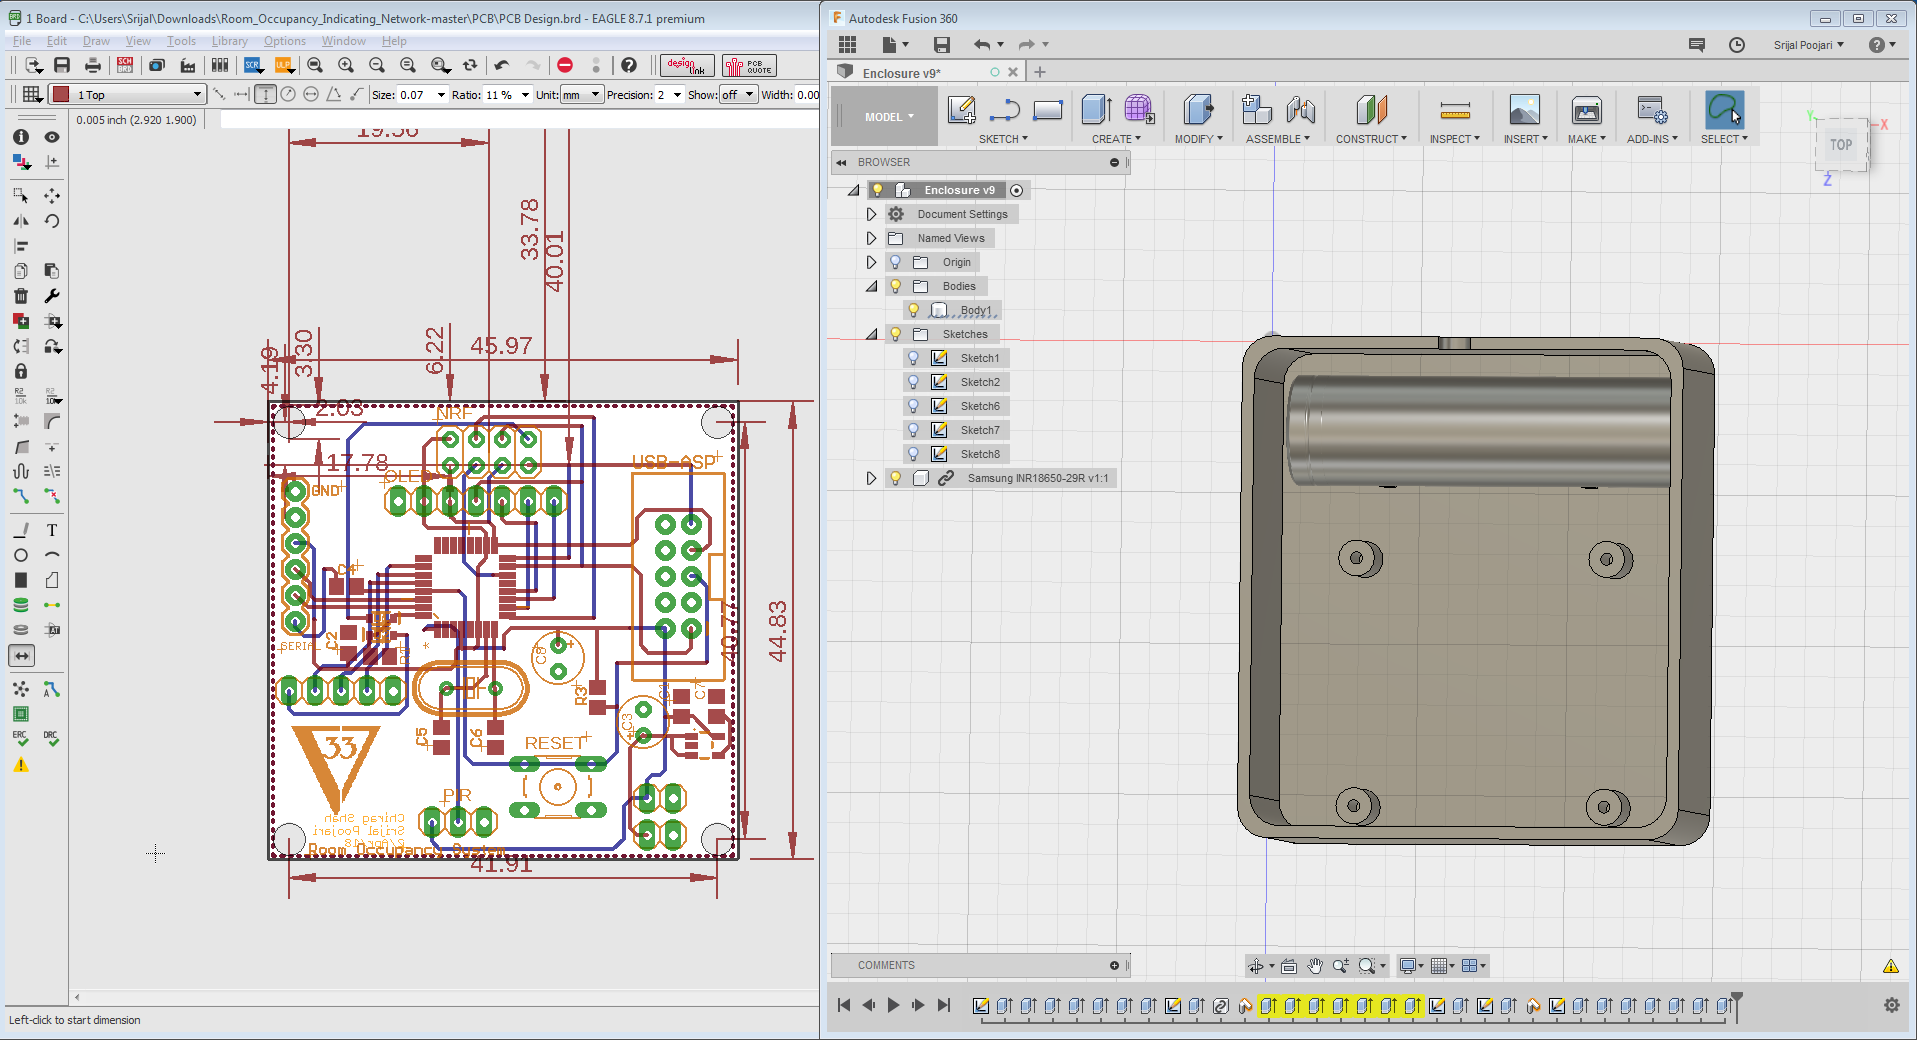
\includegraphics[scale=0.25]{modelling_process.png}
	\\
	\vspace{10pt}	
	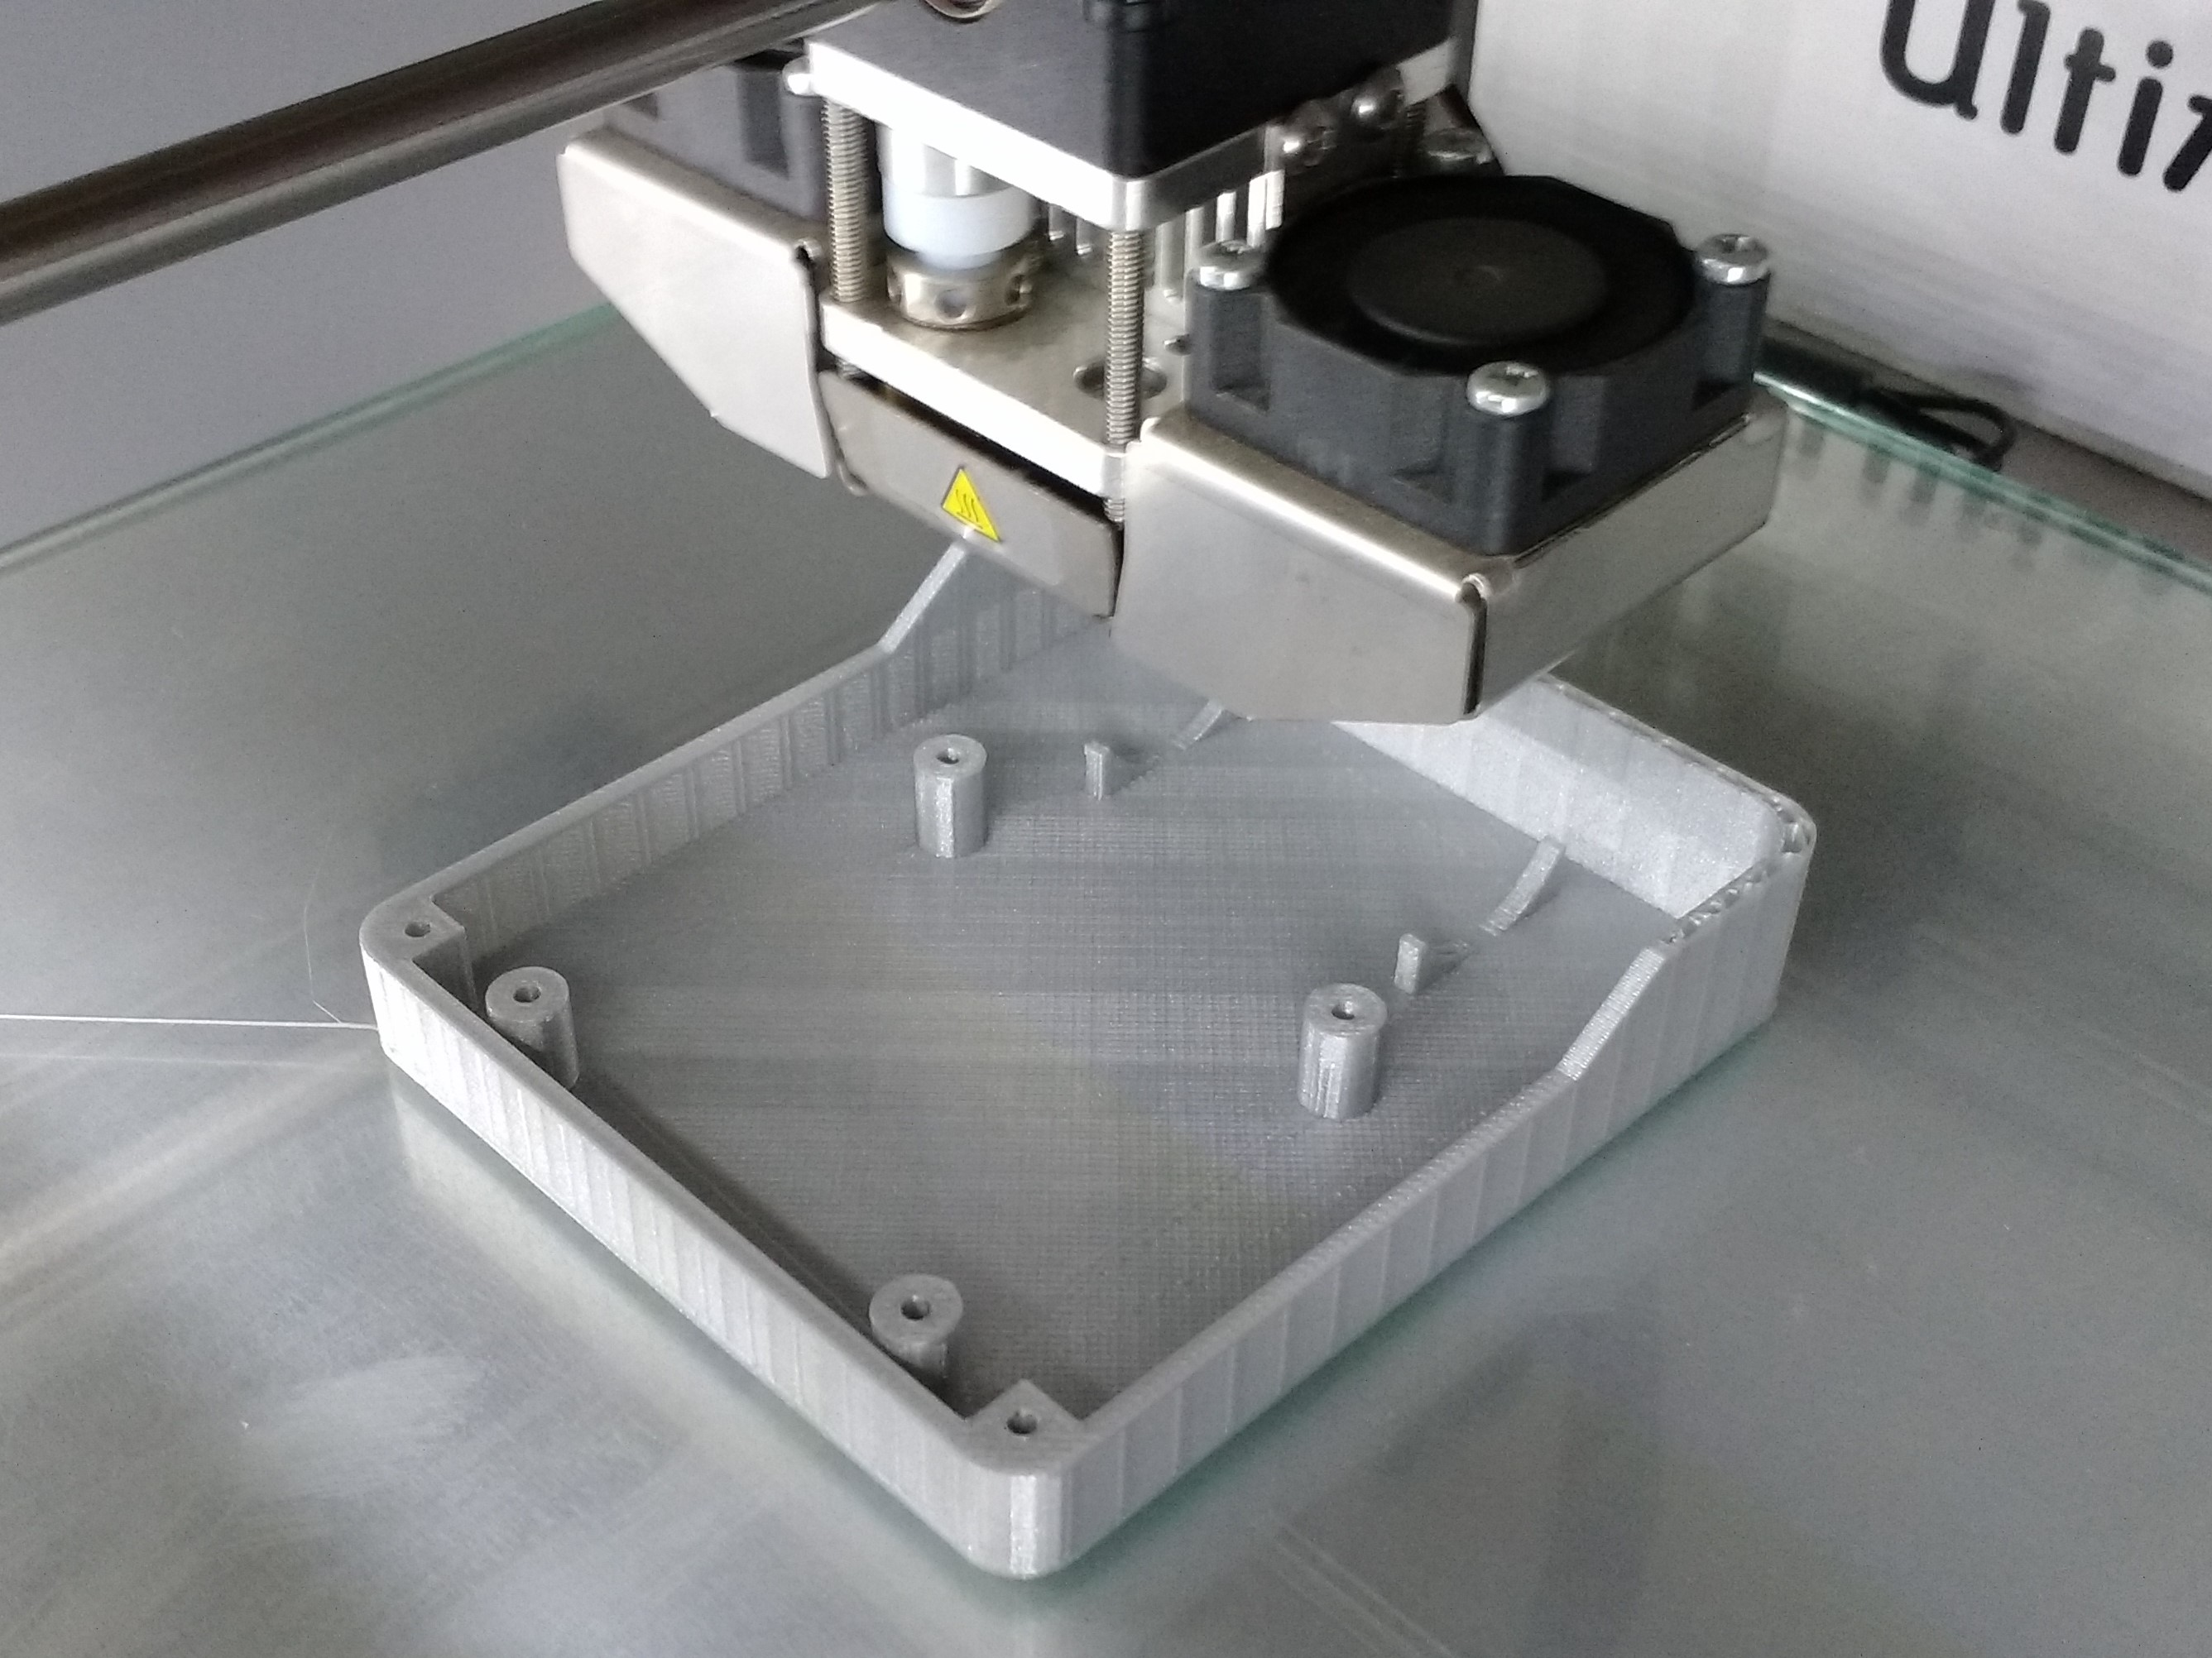
\includegraphics[scale=0.065]{3DPrint.jpg}
	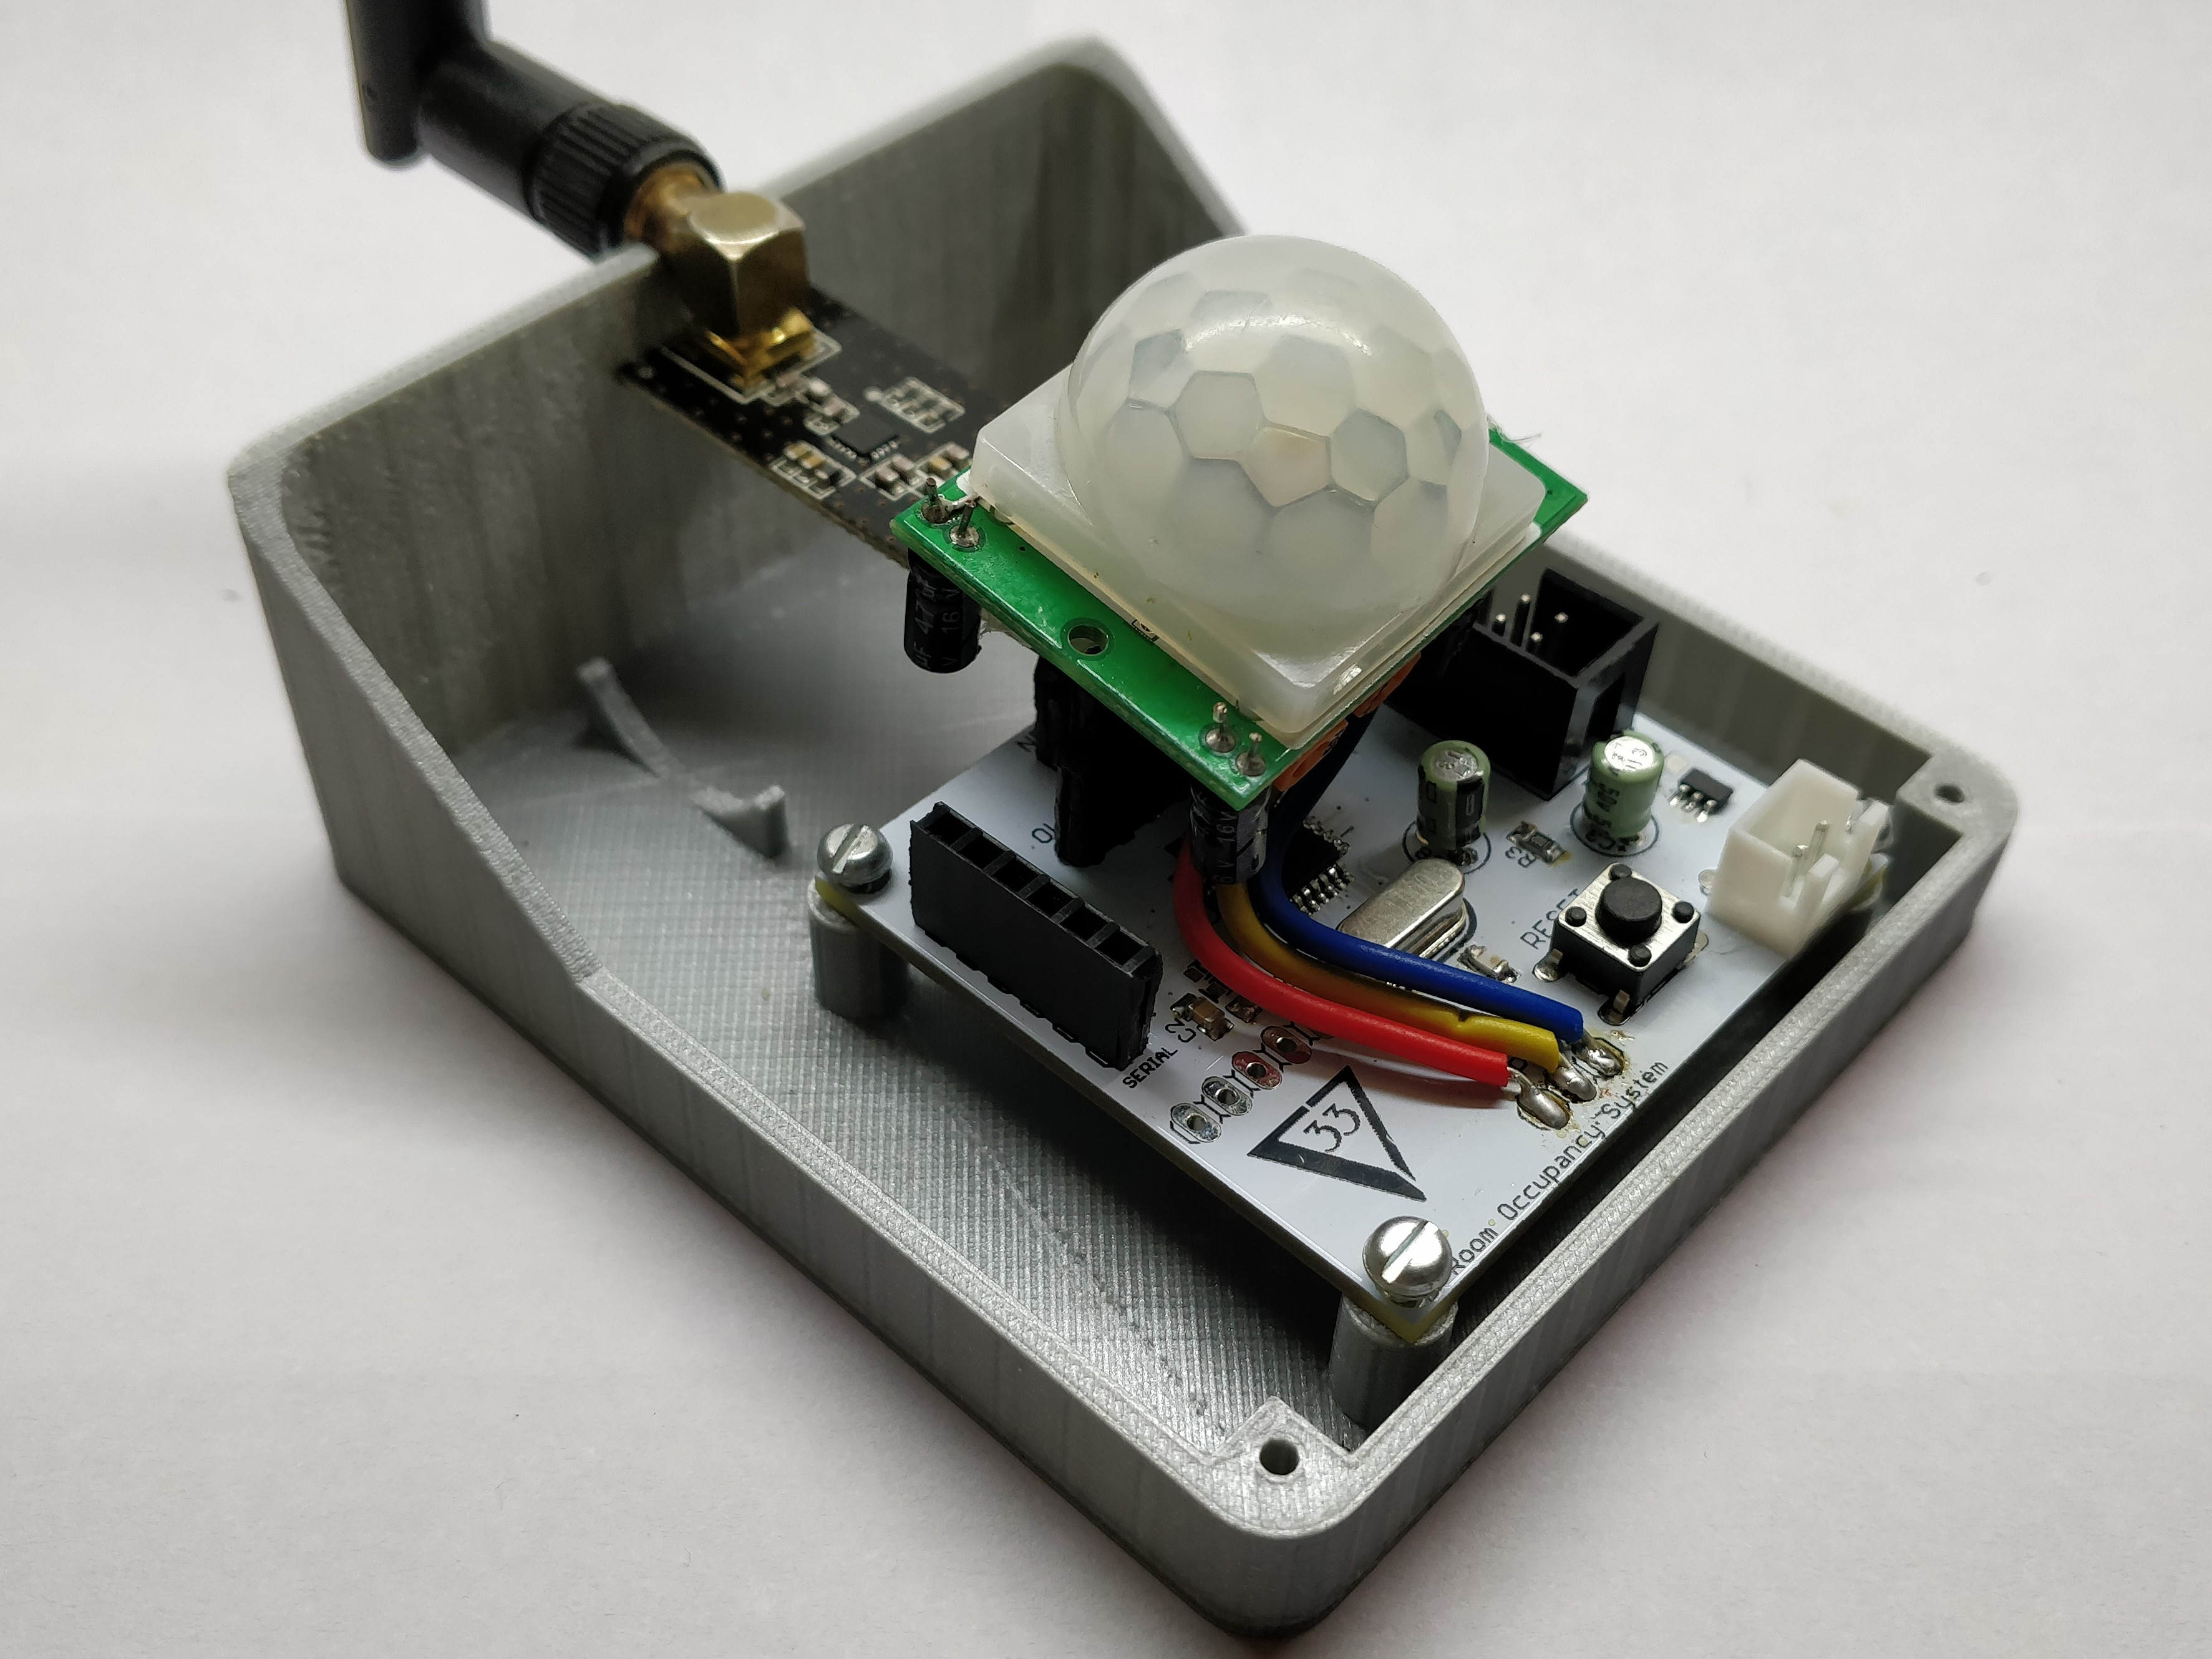
\includegraphics[scale=0.05]{AssemPCB2.jpg}
\end{center}

\section{Interface with Master Node and Web-GUI}
All packets sent from each sensor node are eventually routed to the master node, which relays it to the computer maintaining the web server. The interface between the master node and the computer is done Serially, at a baud rate of 115200 bps. The computer runs a Python script which receives all the sensor data and updates the data on the web server, which displays it to the client (browser). Timestamps are passed between the the web server and client in Unix Epoch format, while a more precise timestamp is logged locally to a text file. 
Real-time information of all the sensor nodes had to be displayed in a easy to interpret format for the user. In case of Occupeye, the sensor information is displayed on top of the map of the room itself, which makes it incredibly easy to interpret. 
\begin{center}
	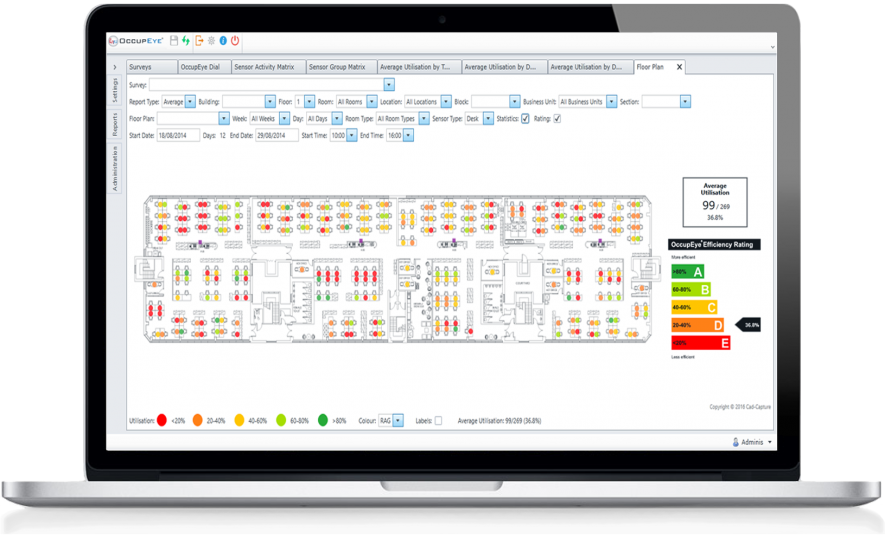
\includegraphics[scale=0.5]{occupeye_map.png}
\end{center}
Since, this is a demonstration model, and since the number of nodes is less, we do not have a fixed outline of a room available so the sensor information is just displayed on a simple browser based GUI.
The webserver was created using the Flask micro web framework, based off Python, and the client end was designed using HTML, CSS and Javascript. High speed dynamic connection between the client and server is implemented using Socket.IO. The MomentJS javascript library was used for timestamping and does the timekeeping on the client end.

\begin{center}
	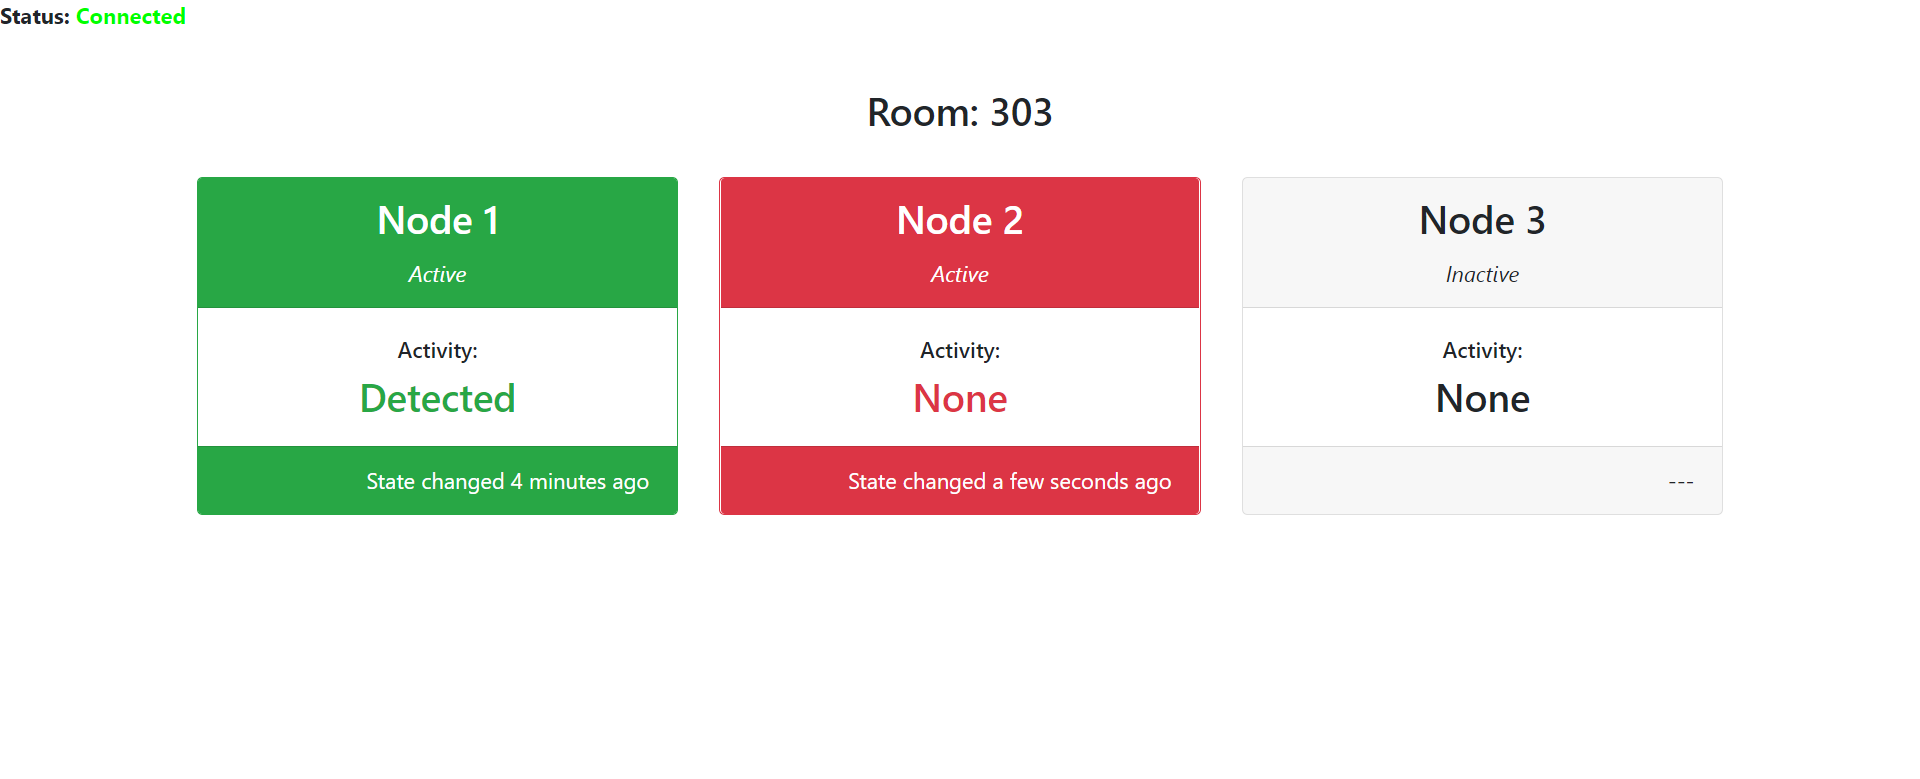
\includegraphics[scale=0.4]{Website1.png}
	\\
	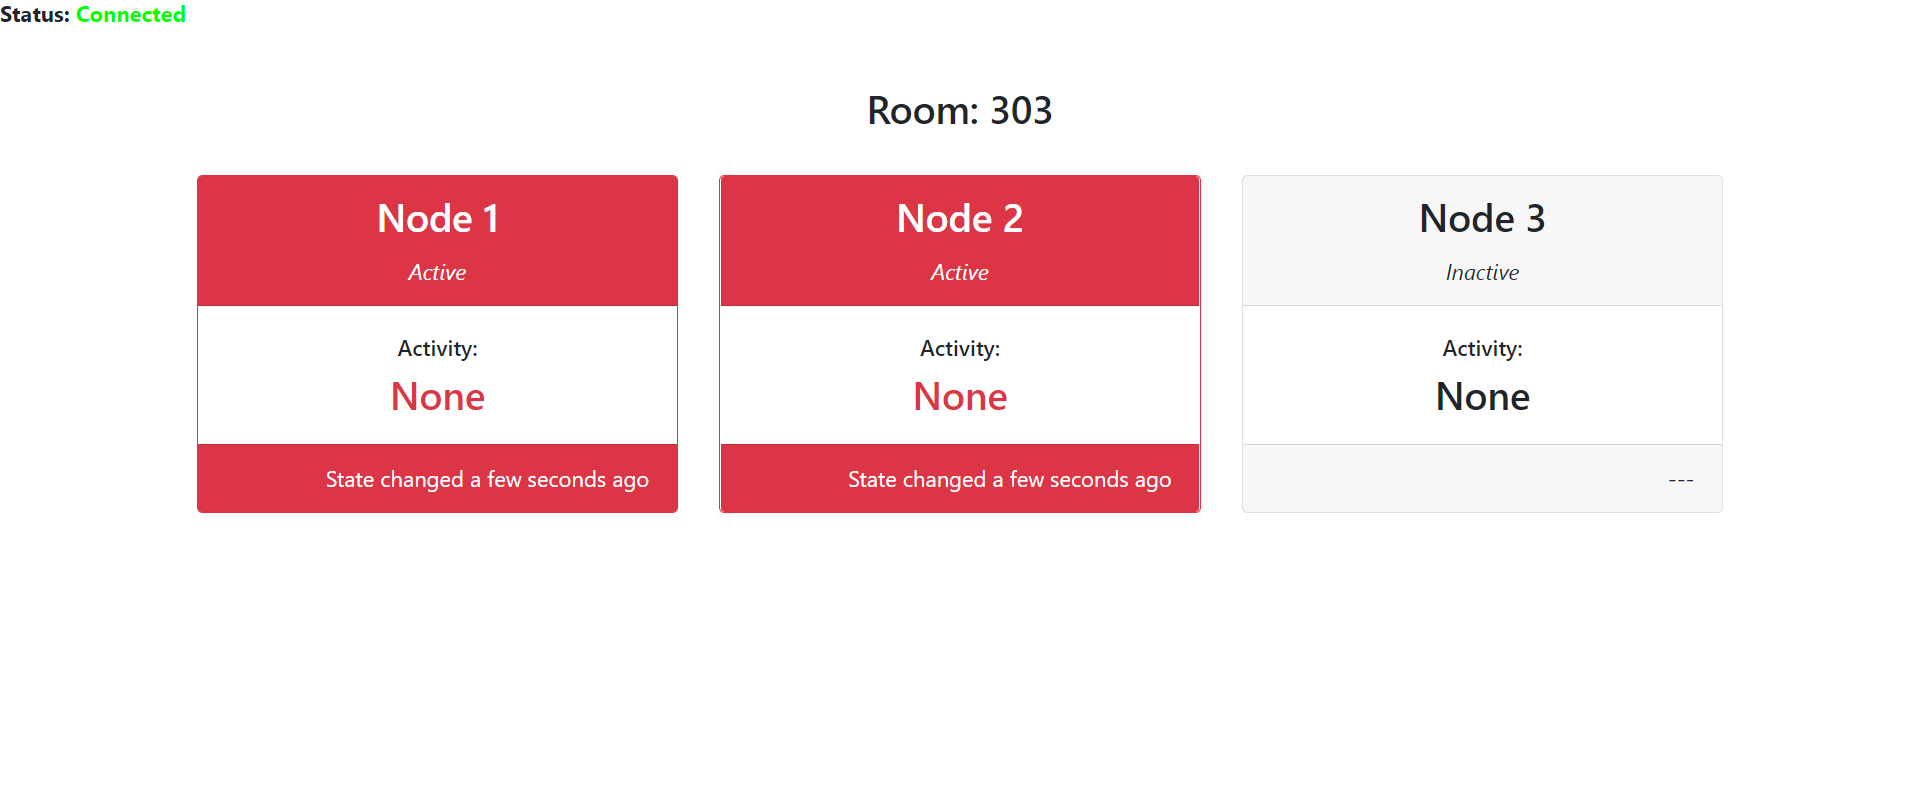
\includegraphics[scale=0.4]{Website2.png}
	%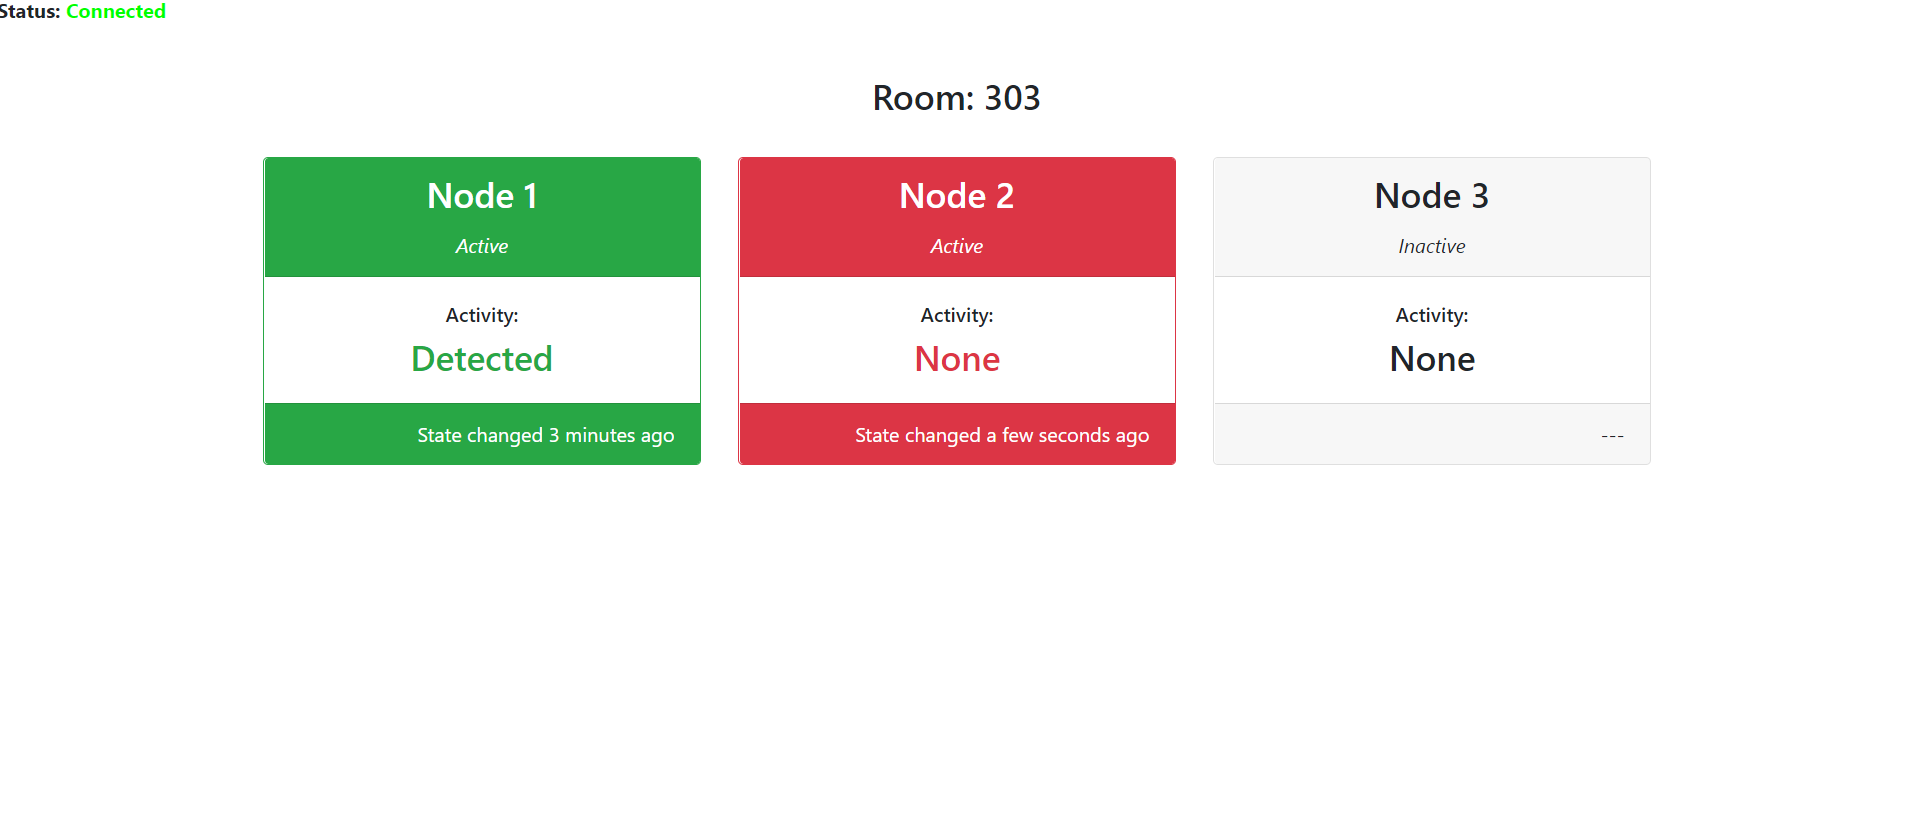
\includegraphics[scale=0.25]{Website3.png}
\end{center}
